\documentclass[11pt]{article}
\usepackage[a4paper, margin=20mm]{geometry}
\usepackage{hyperref}

\usepackage{amsmath}
\usepackage{physics}

\usepackage{graphicx}
\graphicspath{ {./figs/} }
\usepackage{subfig}

%\renewcommand{\baselinestretch}{2}
\usepackage{setspace}
\doublespacing
\usepackage{titlesec}
\usepackage{authblk}
\usepackage{titling}
\usepackage[backend=biber,
style=authoryear,
citestyle=apa]{biblatex}
\addbibresource{Reference.bib} % The filename of the bibliography

\usepackage{enumitem}

\titlespacing\section{0pt}{0pt plus 0pt minus 0pt}{0pt plus 2pt minus 2pt}
\titlespacing\subsection{0pt}{0pt plus 4pt minus 2pt}{0pt plus 2pt minus 2pt}
\titlespacing\subsubsection{0pt}{0pt plus 4pt minus 2pt}{0pt plus 2pt minus 2pt}

\usepackage{amsfonts}
\newtheorem{theorem}{Definition}

\begin{document}

\begin{titlepage} % Suppresses displaying the page number on the title page and the subsequent page counts as page 1
	\newcommand{\HRule}{\rule{\linewidth}{0.5mm}} % Defines a new command for horizontal lines, change thickness here
	
	\center % Centre everything on the page
	
	%------------------------------------------------
	%	Headings
	%------------------------------------------------
	
	\textsc{\LARGE University of Oxford}\\[1.5cm] % Main heading such as the name of your university/college
	
	\textsc{\Large Engineering Science}\\[0.5cm] % Major heading such as course name
	
	\textsc{\large 4YP Report}\\[0.5cm] % Minor heading such as course title
	
	%------------------------------------------------
	%	Title
	%------------------------------------------------
	
	\HRule\\[0.4cm]
	
	{\huge\bfseries The Future of Work}\\[0.4cm] % Title of your document
	
	\HRule\\[1.5cm]
	
	%------------------------------------------------
	%	Author(s)
	%------------------------------------------------
	
	\begin{minipage}{0.4\textwidth}
		\begin{flushleft}
			\large
			\textit{Author}\\
			Terence \textsc{Tan} % Your name
		\end{flushleft}
	\end{minipage}
	~
	\begin{minipage}{0.4\textwidth}
		\begin{flushright}
			\large
			\textit{Supervisor}\\
			Professor Michael A \textsc{Osborne} % Supervisor's name
		\end{flushright}
	\end{minipage}
	
	% If you don't want a supervisor, uncomment the two lines below and comment the code above
	%{\large\textit{Author}}\\
	%John \textsc{Smith} % Your name
	
	%------------------------------------------------
	%	Date
	%------------------------------------------------
	
	\vfill\vfill\vfill % Position the date 3/4 down the remaining page
	
	{\large\today} % Date, change the \today to a set date if you want to be precise
	
	%------------------------------------------------
	%	Logo
	%------------------------------------------------
	
	\vfill\vfill
	
\includegraphics[width=0.5\textwidth]{Figures/logo.png}\\[1cm] % Include a department/university logo - this will require the graphicx package
	 
	%----------------------------------------------------------------------------------------
	
	\vfill % Push the date up 1/4 of the remaining page
	
\end{titlepage}

\begin{abstract}
We took data from the US Bureau of Labor Statistics\footnote{https://www.bls.gov} (BLS) regarding age distribution within occupations in the United States from the year 2011 to 2021, and preprocessed it according to the 2018 Standard Occupational Classification System so as to standardise the data across the years. We then explore trends within this dataset before merging it with an automatability dataset containing information about the Probability of Computerisation for occupations. We found no correlations between the rate of ageing in occupations and their Probability of Computerisation. However, we did find a promising relationship between the proportion of 55 years and older in occupations and the Probability of Computerisation. Assuming this trend is statistically significant, it suggests that occupations at higher risk of automation tend to have a lower proportion of workers who are 55 years and older. We applied a number of linear regression techniques on the joint dataset to further investigate this trend. We then used Probably Approximately Correct Learning in a novel way to perform statistical analysis on the joint dataset, which acts as a proof of concept of using such a technique in combination with a scenario discarding scheme to deal with outliers in datasets. That being said, more needs to be done to determine the statistical significance of this trend. Hence, we offer no guarantees that automation can make up for the shrinking labour force due to an ageing population, and recommend governments take a more active approach in managing the effects of automation and an ageing population.
\end{abstract}

   

\section*{Acknowledgements}

	\thispagestyle{empty}
   I would like to express my deepest gratitude to Professor Michael Osborne for supervising me throughout this project. His insights and guidance are very much appreciated. This project would also not have been possible without the automatability dataset provided by him. Also special thanks to my fellow colleagues who read my drafts and provided invaluable feedback.


\clearpage


\section{Introduction}
\label{sec:Introduction}

Technological advancement is widely believed to be the primary driving force behind economic growth (\cite{RePEc:ssa:lembks:dosietal-1988}). At the same time, there is potential for technological displacement of labour. This concept of 'technological unemployment' was first introduced by David Ricardo in the 19th century (\cite{WoirolGregoryR1997Ttua}), who wrote that he had become "convinced that the substitution of machinery for human labour, is often very injurious to the interests of the class of labourers" (\cite{10.1257/jep.33.2.229}). This idea was further explored by John Maynard Keynes, who blamed "our discovery of means of economising the use of labour outrunning the pace at which we can find new uses for labour" for potential widespread technological unemployment (\cite{Keynes2010}). However, there are those that are cautiously optimistic of the impact of technological advances on labour. Prominent member of the United Automobile Workers union Walter Reuther and his colleague had hopes that automation could eliminate the drudgery of industrial work and ultimately allow workers to pursue leisurely interests. Yet, even they shared fears that automation could lead to widespread structural unemployment if not managed properly (\cite{SteigerwaldDavid2010WRtU}). Alas, history seems to have validated their fears; the proportion of manufacturing employment in the US among non-agricultural workers decreased from 32\% in 1955 to 8\% in 2019 (\cite{rose_2021}). That being said, there is no consensus on the impact of technological advances on the decline of the manufacturing sector relative to other factors such as globalisation and offshoring (\cite{RoseElizabethL.2021TDoU}) (\cite{krugman2019globalization}).

At the same time, ageing population is a social issue that has become increasingly relevant all over the world (\cite{2002Wpa1}). It is expected to lead to a reduction in the labour force of countries, and an increase in social spending \cite{marevsova2015economics}. Given the loss of jobs due to automation and the shrinking of the labour force in many countries, a question naturally arises: can we expect automation to make up for the lack of workers in most jobs?

\subsection{Ageing Population}
\label{subsec:ageingpopulation}

The world population is ageing over the next few decades (\cite{science}). The rising elderly to working age population ratio is increasing and will continue to do so (\cite{WHO}). This trend is known as an ageing population, and will strain the public and social services of many countries around the world (\cite{publicservicesstrain}). As one of the key social challenges facing the world for the next few decades, it would be interesting to examine how an ageing population will affect the economy, and in particular, the job market and the interplay with automation in the workplace. As more workers age out of the workforce, automation is expected to make up for it (\cite{futureofemployment}). In the following sections, we shall first examine the ageing trends in the US as well as other countries, and look into related works on ageing population.

\subsection*{Cross-country comparison}
\label{subsec:crosscountrycomparison}

The United States Census Bureau provides a comprehensive report regarding ageing trends in the US in \cite{vespa2018demographic}. From 2030 onwards, all baby boomers will be over the age of 65. Population growth of the country will also be primarily driven by immigration rather than natural increase (number of births minus number of deaths) beginning that year. The number of people aged 65 and older in the US is expected to increase from 49 million in 2016 to 95 million in 2060. This represents an increase in the share of people aged 65 and older from 15\% in 2016 to nearly 25\% of the total US population in 2060. By 2030, 20\% of the US population will be 65 years and older. The number of people aged 85 and older is expected to increase from 6.4 million in 2016 to 19 million in 2060. This represents an increase in the share of people aged 85 and older from about 2\% in 2016 to about 4.7\% of the total US population in 2060.

China is currently home to the largest population of older people in the world (\cite{lancet2022population}), and is expected to age rapidly over the next few decades (\cite{BeardsonTimothy2021Ag:C}). The number of people aged 60 and older will increase from 254 million people in 2019 to 402 million people in 2040; this would be about 28\% of the population in China. (\cite{whochina}). Given that \cite{whochina} showed that around 75\% of people aged 60 and older in China suffer from noncommunicable diseases such as diabetes, the healthcare system in the country can be expected to be put under increasing pressure in the coming decades. Indeed,  \cite{LuoYanan2021TaCf} recommended pushing for more flexible and innovative population health strategies. That being said, the same study also provided some evidence of declining disease burden as well as healthy ageing.

Japan currently has the highest proportion of elderly citizens in the world (\cite{kyodo_2019}). In fact, 28\% of the population is 65 and older. By 2036, this age group will represent about 33\% of the population in Japan (\cite{d2020japan}). \cite{d2020japan} also highights the various socioeconomic impacts of an ageing population in Japan, including a worsening economy and higher expenditure on healthcare. \cite{ParsonsAlexanderJ.Q.2018Aeof} provides evidence that fertility- and migration-based policies are unlikely to reverse the ageing trend in Japan significantly, and recommends improving work productivity of its population and increasing participation rate of senior citizens in the labour force.

The above three countries are currently the three largest economies in the world (\cite{worldbankgdp}). The effects of an ageing population in these countries on their economies will be felt by the world. As it stands, Japan is currently the most 'aged' society among the three, with the US being the 'youngest'. As the country most ahead of the curve in terms of an ageing society, Japan will be closely observed by other countries as a case study of what will transpire in the coming decades.


\subsection*{Related Works}
Research into the social implications of an ageing population had been carried out as far back as 2002. \cite{tinker2002social} outlined the demographic trends around the turn of the millennium that pointed to the future of an ageing world, and highlighted the falling potential support ratio (ratio of people aged 15-64 to people aged 65 and above) around the world, which will affect the distribution of resources, such as in the case of pensions, of a country. This study also talked about the relative power between the young and old, and pointed out that the older generation will have larger share of votes, potentially wielding more political power. Indeed, contemporary authors, such as \cite{Munger+2022}, have noted this power struggle between the older and younger generations. The US government has also been described as a gerontocracy (\cite{noah_2019}) (\cite{thompson_2020}) in modern times. The numbers back this up, with the average age of a US senator being 64 in 2021 (\cite{manning_2022}).

\cite{Cheng2020} conducted a global analysis of population ageing and mortality between 1990 and 2017, and concluded that there was a pattern of higher disease-related deaths due to population ageing around the world within that time period. The study recommended policies aimed at encouraging healthy ageing. Indeed, there is evidence to suggest that the healthcare system in the US is not prepared to meet the increasing demands of the ageing population (\cite{foley_retooling_2020}).



% While this paper will be focusing on the US, there are numerous other studies looking into ageing population of the US as well as other countries and regions of the world. China is expected to age rapidly over the next few decades (\cite{BeardsonTimothy2021Ag:C}), and studies such as \cite{LuoYanan2021TaCf} examined this phenomenon in the context of the country.

\subsection{Project Overview}
\label{subsec:projectoverview}
In this project, we aim to examine the relationship between the age distribution within occupations and the Probability of Computerisation\footnote{Defined as 'job automation by means of computer-controlled equipment' by \cite{osborne2017future}} (calculated by \cite{futureofemployment}) of those occupations, and apply statistical techniques on any significant trends that we may find. This project is motivated by the question of whether automation can solve the problem of ageing population and vice versa. We will go into further detail about the data and where we got them from in Chapter \ref{sec:Dataset}. Although similar work has been done on this topic (\cite{twinthreats}), the study only looked at broad categories of employment. In this project, we zoomed in to look at specific occupations. Other papers (\cite{10.1257/aer.p20171101})(\cite{10.1371/journal.pone.0263704}) examined the effects of ageing population and automation on the labour market. In particular, \cite{10.1371/journal.pone.0263704} went one step further and took into account the interaction effects of ageing population and automation as well. However, as far as we can tell, we are the first to directly examine the relationship between automation and distribution of age within occupations at such a detailed scale. This was all be done using Python, with the statistical models implemented using the scikit-learn library\footnote{https://scikit-learn.org/stable/}. Specifically, we used a number of linear regression models in Chapter \ref{subsec:Linear Regression}, and applied a Probably Approximately Correct Learning model in a novel manner on a set of data in Chapter \ref{subsec:PAC}.

%look at a Bayesian non-parametric machine learning technique known as Gaussian Process (\cite{GaussianProcess}); this model was used in previous work (\cite{futureofemployment}), and so, would be a good model to start with. We will test and validate against different models and pick the best performing ones.

We will be using the proportion of elderly people as a metric for measuring the `age' of occupations. We acknowledge that the definition of elderly age varies across different countries and cultures (\cite{ageingculture}), and that the ageing process varies for different people depending on a variety of factors (\cite{levine2013modeling})(\cite{hayflick2007biological}). In fact, there are studies looking into moving beyond using chronological age to define an elderly person (\cite{KotterGrhn2015})(\cite{SOTOPEREZDECELIS2018e305})(\cite{klemera2006new}). However, there are numerous issues surrounding this approach (\cite{jylhava2017biological}), such as validation of such results are often difficult (\cite{biologicalagedifficult}), resulting in little consensus on an alternative metric to chronological age. For this reason, we will stick to the conventional definition of 65 years and older as `elderly' (\cite{who2010definition})(\cite{orimo2006reviewing})(\cite{oecddata}). This definition is also convenient for us since the oldest age group featured in our datasets are 65 years and older. Hence, it would make sense to have the metric for measuring the `age' of an occupation be the ratio of people aged 65 years and older to the total number of people in that particular occupation. We will refer to this metric as the Elderly Proportion (EP). However, we also recognise that this definition of 'elderly' coincides with the retirement age of the US (\cite{MunnellAliciaH2013SSRR}). Hence, using this metric alone might lead to misleading results since we would expect people in that age group to leave the workforce. It might be better to use the proportion of 55 years and older as a metric, i.e. the ratio of people aged 55 years and older to the total number of people, since this figure might be more robust to the effects of retirement on labour force participation. We shall refer to this metric as the Old Proportion (OP). Having said that, the Elderly Proportion would still prove to be an interesting metric to investigate. For example, if there is a general trend of increasing EP over the years, that would be a sign of an ageing labour force in spite of the effects of retirement. Therefore, we shall examine both of these metrics in this paper.

\subsection*{Related Works}

\cite{futureofemployment} and \cite{osborne2017future} used data from the Occupational Information Network\footnote{https://www.onetonline.org} (O*NET) as well as hand-labelled data by experts to calculate the Probability of Computerisation for 702 detailed occupations. It was also predicted that 47\% of employment in the US were at risk of computerisation. \cite{pajarinen2015computerization} used the same methodology to show that about 33\% of employment in Finland and Norway are at risk of computerisation. \cite{fuei2017automation} did the same for Singapore, and found that 25\% of employment in the city-state were at high risk of computerisation. Similarly, \cite{brzeski2015roboter} extended the analysis to Germany and concluded that 59\% of employment are at risk of computerisation.

\cite{10.1257/aer.p20171101} showed that there is no inverse relationship between ageing population and economic growth, i.e. an ageing population does not negatively affect the economy. The paper argues that countries that are ageing more rapidly tend to embrace and faster implement automation technologies.

\cite{twinthreats} mapped data from \cite{osborne2017future} to occupations defined under the United Nations' International Standard Classification of Occupations\footnote{https://www.ilo.org/public/english/bureau/stat/isco/} (ISCO), in order to estimate the risk of automation to older workers across 15 countries. The report found that older workers were at medium to high risk of being displaced by automation in several countries. Countries with higher rates of ageing also face the highest risk of automation. Ultimately, the paper encourages discussions around the challenges faced by older workers, in order to enable them to remain in the labour force in light of the decreasing proportion of younger workers.

\cite{10.1371/journal.pone.0263704} used the Probability of Computerisation data calculated by \cite{osborne2017future} and data about age-related abilities from O*NET to examine the interaction effects of computerisation and ageing population on the US labour market in terms of employment growth and earnings growth. The latter two are obtained from the Bureau of Labor Statistics, giving a complete dataset consisting of 501 occupations. The paper found that both computerisation and ageing population have significant effects on employment growth but not earnings growth. Specifically, the higher the Probability of Computerisation, the lower the employment growth. This is also supported by \cite{graetz2018robots} and \cite{acemoglu2020robots}. The paper also found that the strength of the relationship between the Probability of Computerisation and employment  growth is dependent on age-related abilities required for the particular occupation.

\newpage

\section{Dataset}
\label{sec:Dataset}
We used two main metrics for this project: the Probability of Computerisation of occupations, and the age distribution within occupations. The dataset for the former is provided in an earlier work by \cite{futureofemployment}. The latter can be found in datasets provided by the US Bureau of Labour Statistics; there is one dataset for each year from 2011 to 2021. All the datasets mentioned above use the Standard Occupational Classification (SOC) to classify the occupations, which means that we can map from one dataset to the another using the SOC codes\footnote{https://www.bls.gov/soc/2018/soc\_structure\_2018.pdf}. However, it is necessary to perform some data wrangling before we can proceed with the mapping. Additionally, changes were made to the SOC in 2018, so we would have to standardise all the datasets. In the following sections, we shall examine the datasets and the required data wrangling in more detail.

\subsection{BLS Dataset}
\label{subsec: BLS}
As mentioned in Chapter \ref{sec:Dataset}, the BLS provides one dataset for each year from 2011 to 2021. The datasets from 2011 to 2019 follow the old SOC while the 2020 and 2021 ones follow the updated version. We want to standardise everything according to the updated SOC. We first label each dataset with the respective year and concatenate  all of them along the row axis; we shall refer to this concatenated dataset as the BLS dataset for the rest of the paper. A section of the BLS dataset can be seen in Figure \ref{fig:df}. Note that the numbers under the \emph{Total} and age group columns are in thousands. Furthermore, the median age is not provided for all occupations, which makes it less useful as a metric. Hence, we will not be using it in this paper.

\begin{figure}[!htb]
    \centering
    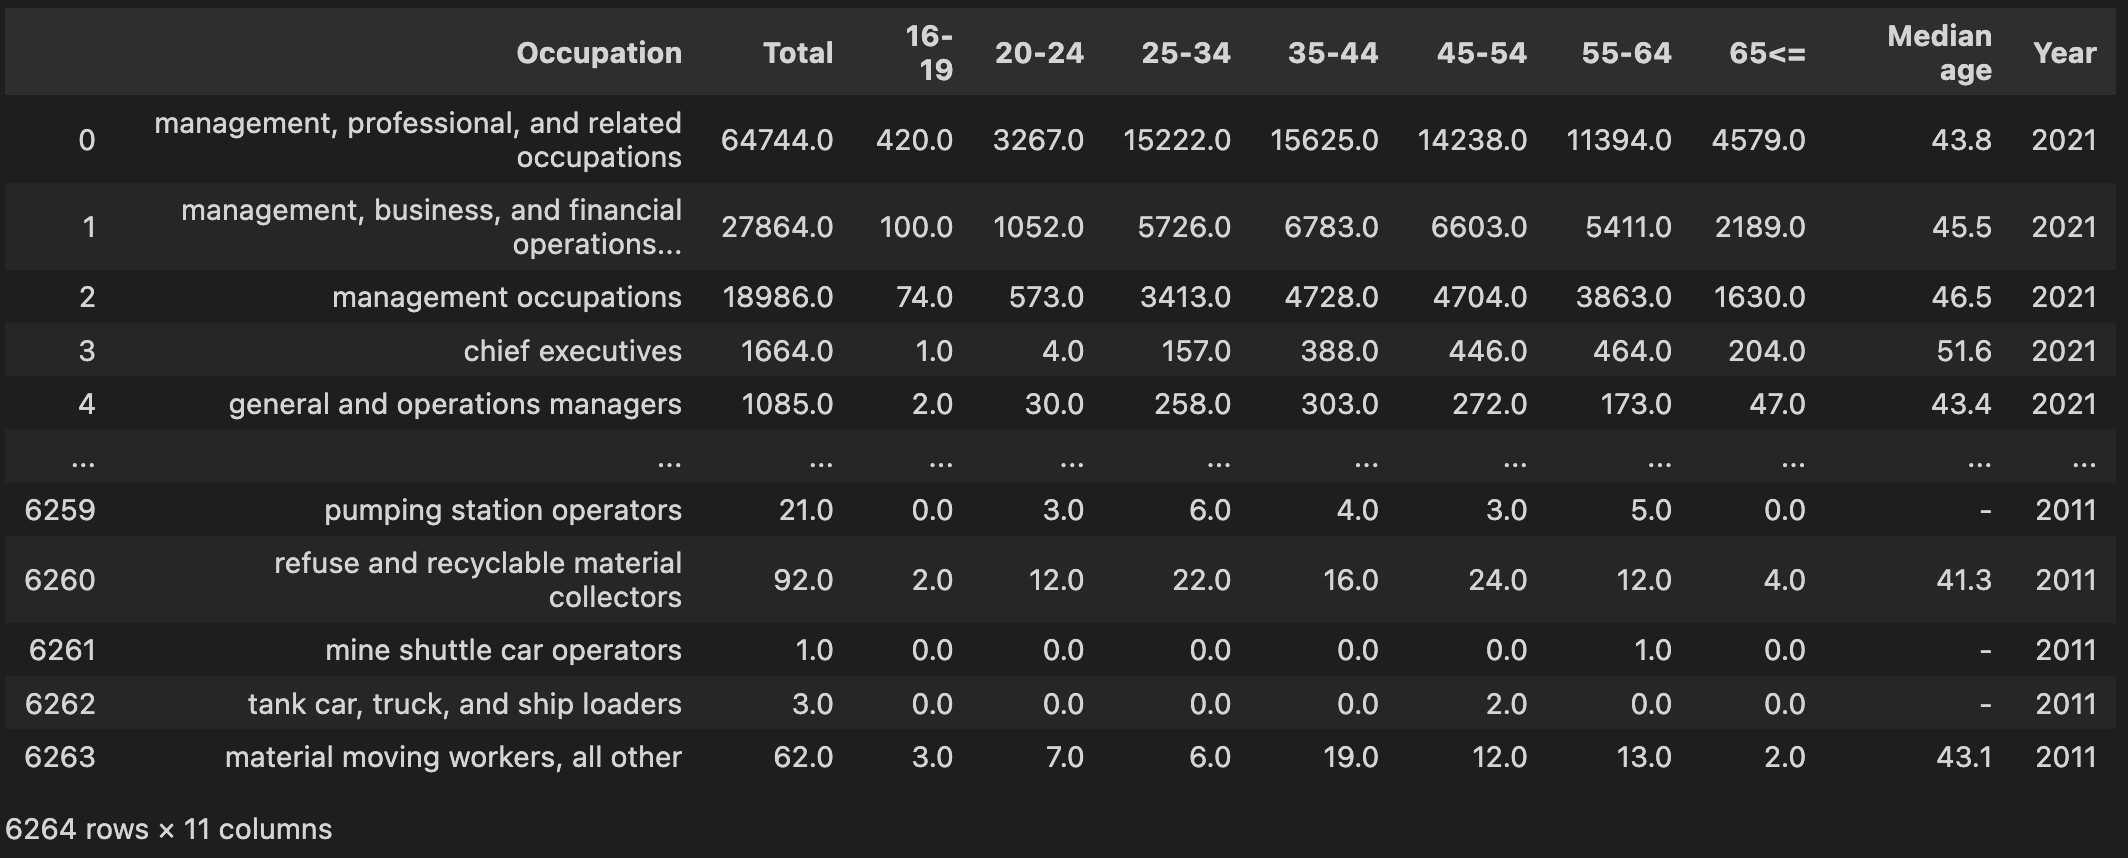
\includegraphics[width=12cm]{Figures/BLS dataset (before).png}
    \caption{BLS dataset (before processing)}
	\label{fig:df}
\end{figure}

While the BLS did provide documents\footnote{https://www.bls.gov/soc/2018/home.htm} outlining and explaining the changes to the SOC, it is generally too vague to be anything more than a rough guide. Furthermore, some of the changes made to the SOC are fairly complex. In addition to that, the BLS collected data differently for some occupations after 2019. For example, both `Marketing Managers' (SOC code: 11-2021) and `Sales Managers' (SOC code: 11-2022) are classified under `Marketing and Sales Managers' (SOC code: 11-2020). From 2011 to 2019, the BLS only collected data for `Marketing and Sales Managers' while they collected data for `Marketing Managers' and `Sales Managers' separately in 2020 and 2021. While this represents more detailed data, it is inconsistent with data collected in previous years.

In order to list out all the changes and inconsistencies, we use the \emph{pandas.DataFrame.join} function to join an old SOC dataset (from 2011 to 2019) with an updated SOC dataset (from 2020 to 2021) using the \emph{Occupation} column. We can then obtain a list of occupations from the old SOC dataset which did not join, and a corresponding list for the updated SOC dataset. We then manually go through both lists and decide on how to standardise the BLS dataset. While this process is tedious, it is reasonably doable since each list only contains about a hundred rows. The changes and rationale for them are listed alongside the occupations in both lists. All of these are placed in an Excel file\footnote{https://github.com/terencetan-c/4YP-The-Future-of-Work/blob/main/Data\%20cleaning/Changes.xlsx}.

The list of actions required are as follows: -, Delete, Change, Combine, Combine but keep. The dash indicates that no action is required. `Delete' means to delete the occupation; this is usually because the particular occupation no longer exists under the new SOC. `Change' indicates a name change. `Combine' indicates that two or more occupations should be combined into the overarching occupation. For example, the two occupations mentioned before, `Marketing Managers' and `Sales Managers', will be combined into `Marketing and Sales Managers' to ensure consistency in the BLS dataset across the years. This will basically be an element-wise addition of the rows, involving only the \emph{Total} and age group columns. This is another reason why we dropped the \emph{Median age} column since we have no way of combining median values for the BLS dataset. Lastly, the `Combine but keep' action is used in cases where we have to combine to maintain consistency but are still able to preserve some granularity by keeping the original rows. For example, the old SOC classifies the four occupations `Home Health Aides' (31-1011), `Psychiatric Aides' (31-1013), `Nursing Assistants' (31-1014), and `Orderlies' (31-1015) under `Nursing, Psychiatric, and Home Health Aides' (31-1000 and 31-1010). Additionally, the old SOC also has `Personal Care Aides' (39-9020 and 39-9021) classified separately. The new SOC renamed `Nursing, Psychiatric, and Home Health Aides' to `Home Health and Personal Care Aides; and Nursing Assistants, Orderlies, and Psychiatric Aides' (and changed the SOC code from 31-1000 to 31-1100) and moved `Personal Care Aides' (now 31-1122) under this newly named occupation. Another thing to note is that the datasets following the old SOC only collected data of `Nursing, Psychiatric, and Home Health Aides' as a whole instead of the four occupations individually. They also collected data for `Personal Care Aides'. On the other hand, the datasets following the new SOC collected data for the four occupations, `Home Health Aides' (now 31-1121), `Psychiatric Aides' (now 31-1133), `Nursing Assistants' (now 31-1131), and `Orderlies' (now 31-1132), and the newly moved occupation, `Personal Care Aides', separately. Note that both groups of datasets have data of `Personal Care Aides' on its own, and we would like to keep it that way to preserve granularity of the data. For the datasets following the old SOC, we would apply `Combine' on `Nursing, Psychiatric, and Home Health Aides' (effectively just a name change in this case) and `Combine but keep' on `Personal Care Aides'. For the new SOC datasets, we apply `Combine' on the four occupations and `Combine but keep' on `Personal Care Aides'. This way, we end up with data for a combined `Nursing, Psychiatric, and Home Health Aides' to `Home Health and Personal Care Aides; and Nursing Assistants, Orderlies, and Psychiatric Aides', while simultaneously still retaining `Personal Care Aides'.

Having systematically gone through all the inconsistencies and indicating one of the five actions required for the inconsistencies, we then use Python to automate the standardisation process. This gives us the standardised BLS dataset.

One more thing to note is that the occupations in the BLS dataset are not labelled with their respective SOC codes. This is easily rectified once the above data wrangling is completed by joining (on \emph{Occupation}) the BLS dataset with the list of SOC codes to map from occupation name to code.

\subsection{Automatability Dataset}

This dataset (which we shall refer to as Automatability dataset) was obtained from \cite{futureofemployment}, and features 702 Detailed Occupations. For each of these occupations, a Probability of Computerisation had been calculated. We shall refer to this probability as PCom. Other variables are included as well, such as the skills associated with each occupation and a Category Label. These were used to calculate the PCom, but we will just focus on the PCom in this paper.

\newpage

\section{Preliminary Findings}
\label{sec:prelim findings}

In order to make sense of how well the BLS dataset represents the US labour force, we plot the ratio of the total labour numbers provided by the BLS dataset for each year to the total US civilian labour force\footnote{https://www.bls.gov/cps/cpsaat01.htm} for that year. We do that for \emph{Major Group}, \emph{Minor Group}, \emph{Broad Group}, and \emph{Detailed Occupation} separately. The resulting plots can be seen in Figure \ref{proportion}. Clearly, \emph{Major Group} occupations are most representative of the US civilian labour force, with \emph{Minor Group} being the least. Looking through the BLS dataset, this makes sense since the BLS tended to mostly collect high-level data (\emph{Major Group}) and low-level data (\emph{Broad Group} and \emph{Detailed Occupation}). Another thing to note is that many \emph{Broad Group} occupations only contain a single \emph{Detailed Occupation} which also shares the same occupation name (for example, \emph{Chief Executives}: 11-1010 and 11-1011). Hence, it is not surprising that the ratios for \emph{Broad Group} and \emph{Detailed Occupation} are so similar.

It is important to consider the fact that the US civilian labour force includes both the employed and the unemployed. In years with unusual levels of unemployment rate, the ratios will be distorted and paint a misleading picture. Indeed, we see in Figure \ref{proportion} that there is a considerable dip in the ratios in 2020 relative to other years, coinciding with the onset of the COVID-19 pandemic (\cite{covid2020unemployment})(\cite{congresscovidunemployment}). Plotting the ratios relative to the employed portion of the US civilian labour force accounts for this; as seen in Figure \ref{proportionemp}, the dip in 2020 is no longer present. We can also see that the unemployment rate did not distort the ratios significantly. Hence, our conclusion from before still holds: the \emph{Major Group} is most representative of the US civilian labour force. With that in mind, we will try to use \emph{Major Group} data as much as possible and exercise caution when using \emph{Detailed Occupation} and \emph{Broad Group} data. As for \emph{Minor Group} data, we will neglect it given its low representation of the labour force.



\begin{figure}[!htb]
	\centering
	\subfloat[Major Group]{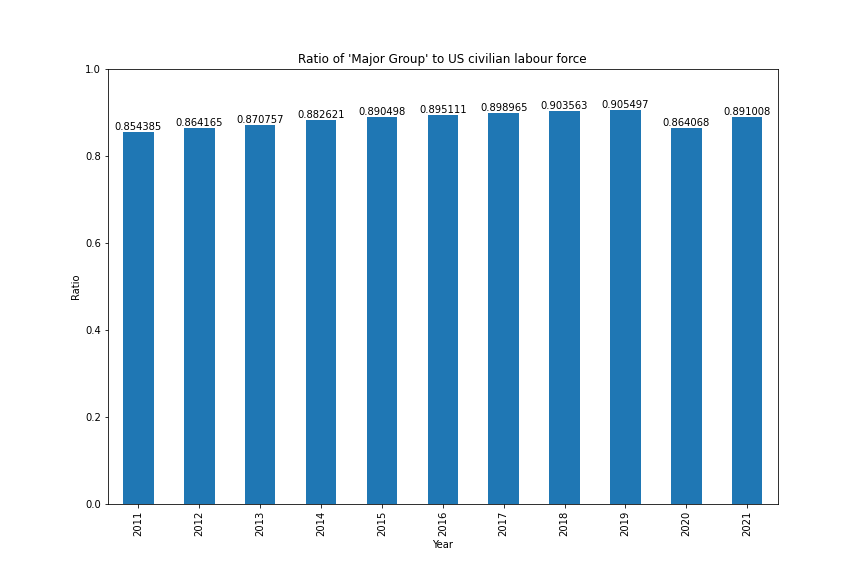
\includegraphics[width=8.5cm]{Figures/Proportion Major.png}\label{fig:promajor}}
	  \hfill
	\subfloat[Minor Group]{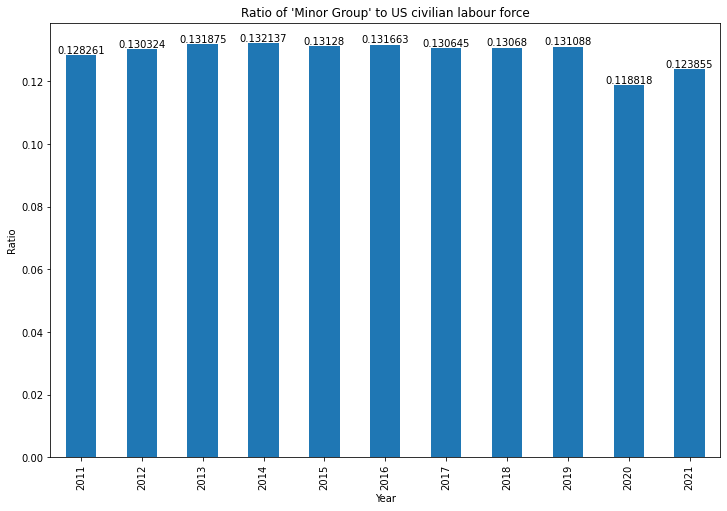
\includegraphics[width=8.5cm]{Figures/Proportion Minor.png}\label{fig:prominor}}
	\hfill
	\subfloat[Broad Group]{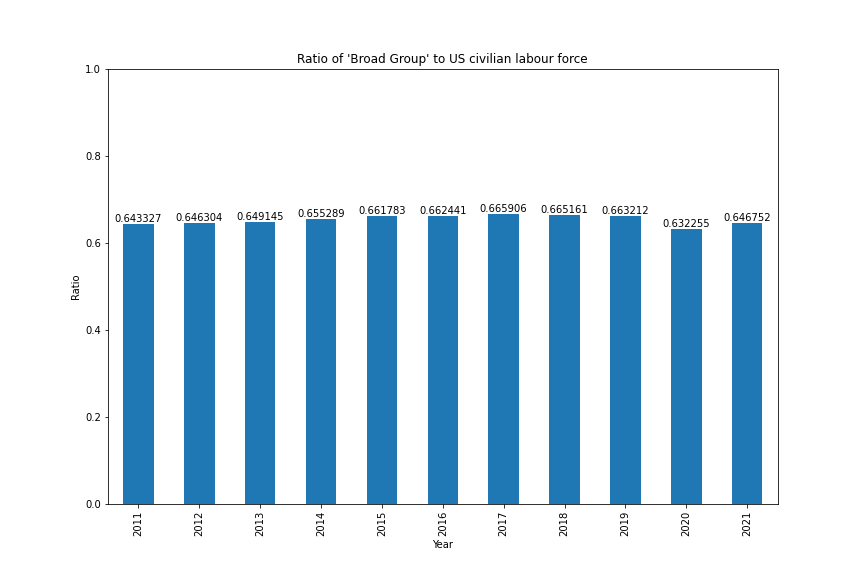
\includegraphics[width=8.5cm]{Figures/Proportion Broad.png}\label{fig:probroad}}
	\hfill
	\subfloat[Detailed Occupation]{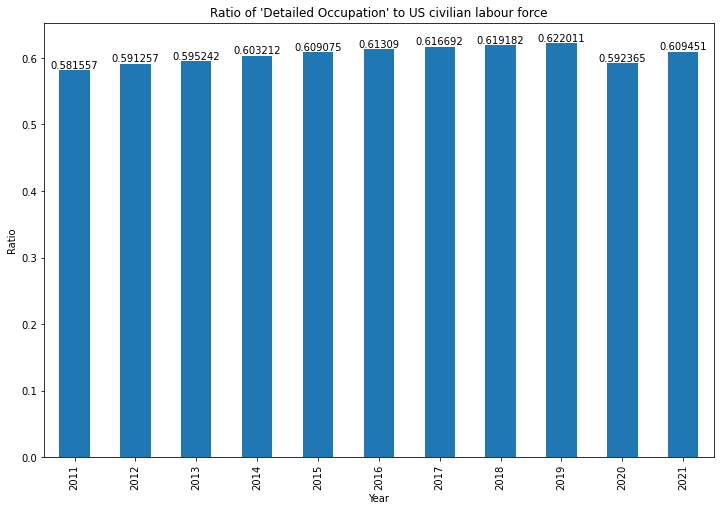
\includegraphics[width=8.5cm]{Figures/Proportion Detailed.png}\label{fig:prodetailed}}
	\hfill
	\caption{Ratio of the various SOC categories to the US civilian labour force}
	\label{proportion}
  \end{figure}
  
\begin{figure}[!htb]
	\centering
	\subfloat[Major Group]{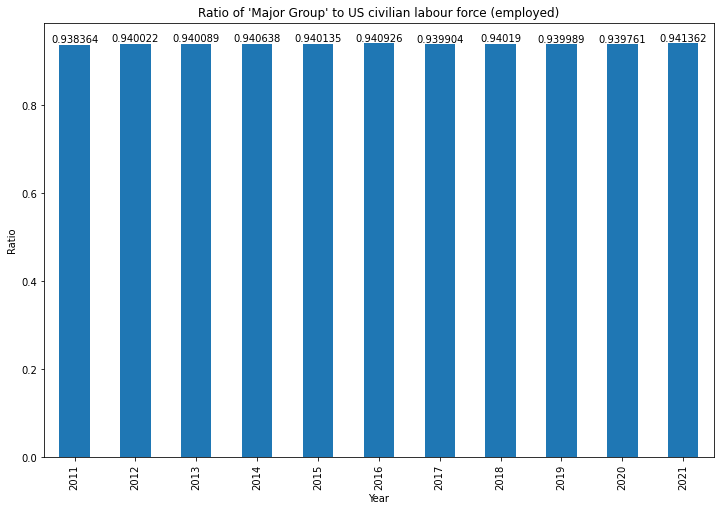
\includegraphics[width=8.5cm]{Figures/Proportion Major (employed).png}\label{fig:empmajor}}
	\hfill
	\subfloat[Minor Group]{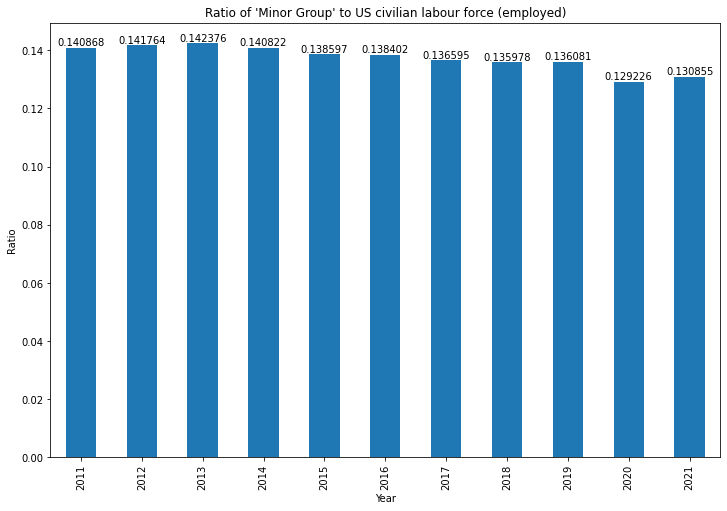
\includegraphics[width=8.5cm]{Figures/Proportion Minor (employed).png}\label{fig:empminor}}
	\hfill
	\subfloat[Broad Group]{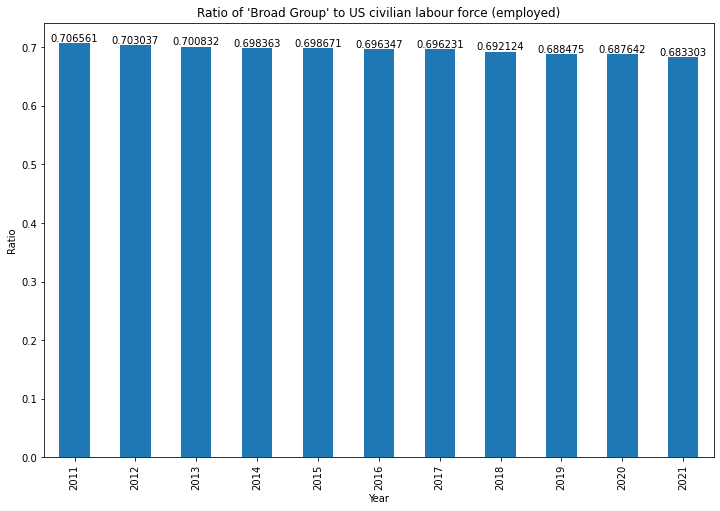
\includegraphics[width=8.5cm]{Figures/Proportion Broad (employed).png}\label{fig:empbroad}}
	\hfill
	\subfloat[Detailed Occupation]{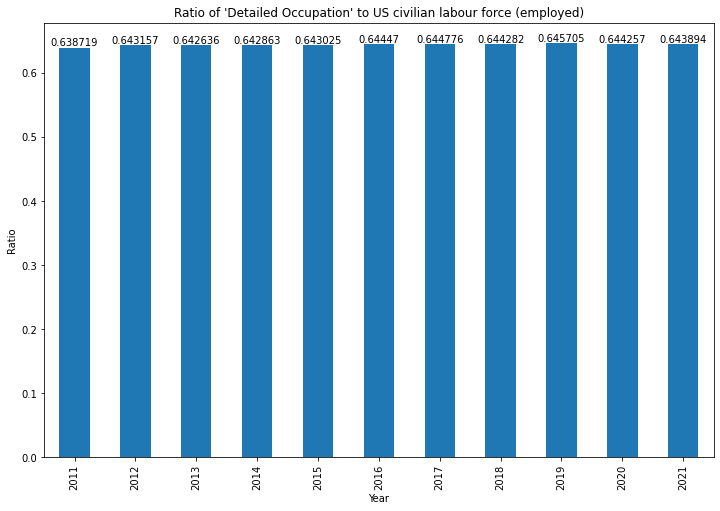
\includegraphics[width=8.5cm]{Figures/Proportion Detailed (employed).png}\label{fig:empdetailed}}
	\hfill
	\caption{Ratio of the various SOC categories to the US civilian labour force (employed)}
	\label{proportionemp}
\end{figure}
    
\subsection{General Trends}
\label{subsec:generaltrends}
We average the EP (refer to Chapter \ref{subsec:projectoverview} for definition) over the Major Groups for each year, and plot the values against the years to obtain Figure \ref{fig:averageEP}. We do the same for OP, and get the plot in Figure \ref{fig:averageOP}. We see a steady increase over the years for both plots, which is not surprising given the ageing population of the US as discussed in Chapter \ref{subsec:crosscountrycomparison}. We can examine these plots in further detail by plotting the EP/OP for each of the 21 Major Groups against the years to obtain Figure \ref{fig:EP/OP against year}; we can see that there is generally an increase across the Major Groups. We do not break down the plots into further detail (for example looking at individual Detailed Occupations) since that will result in plots that are too messy to give us any useful insights.



\begin{figure}[!htb]
	\centering
	\subfloat[Elderly Proportion]{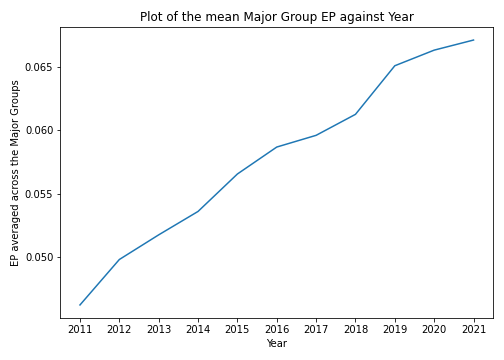
\includegraphics[width=8cm]{Figures/Mean Major Group Elderly Proportion against Year.png}\label{fig:averageEP}}
	\hfill
	\subfloat[Old Proportion]{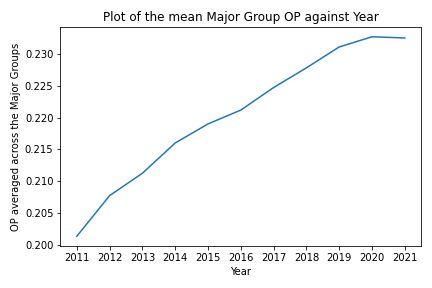
\includegraphics[width=8cm]{Figures/Mean Major Group Old Proportion against Year}\label{fig:averageOP}}
	\hfill
	\caption{Plot of EP/OP (averaged over the Major Groups) against Year}
\end{figure}


\begin{figure}[!htb]
	\centering
	\subfloat[Elderly Proportion]{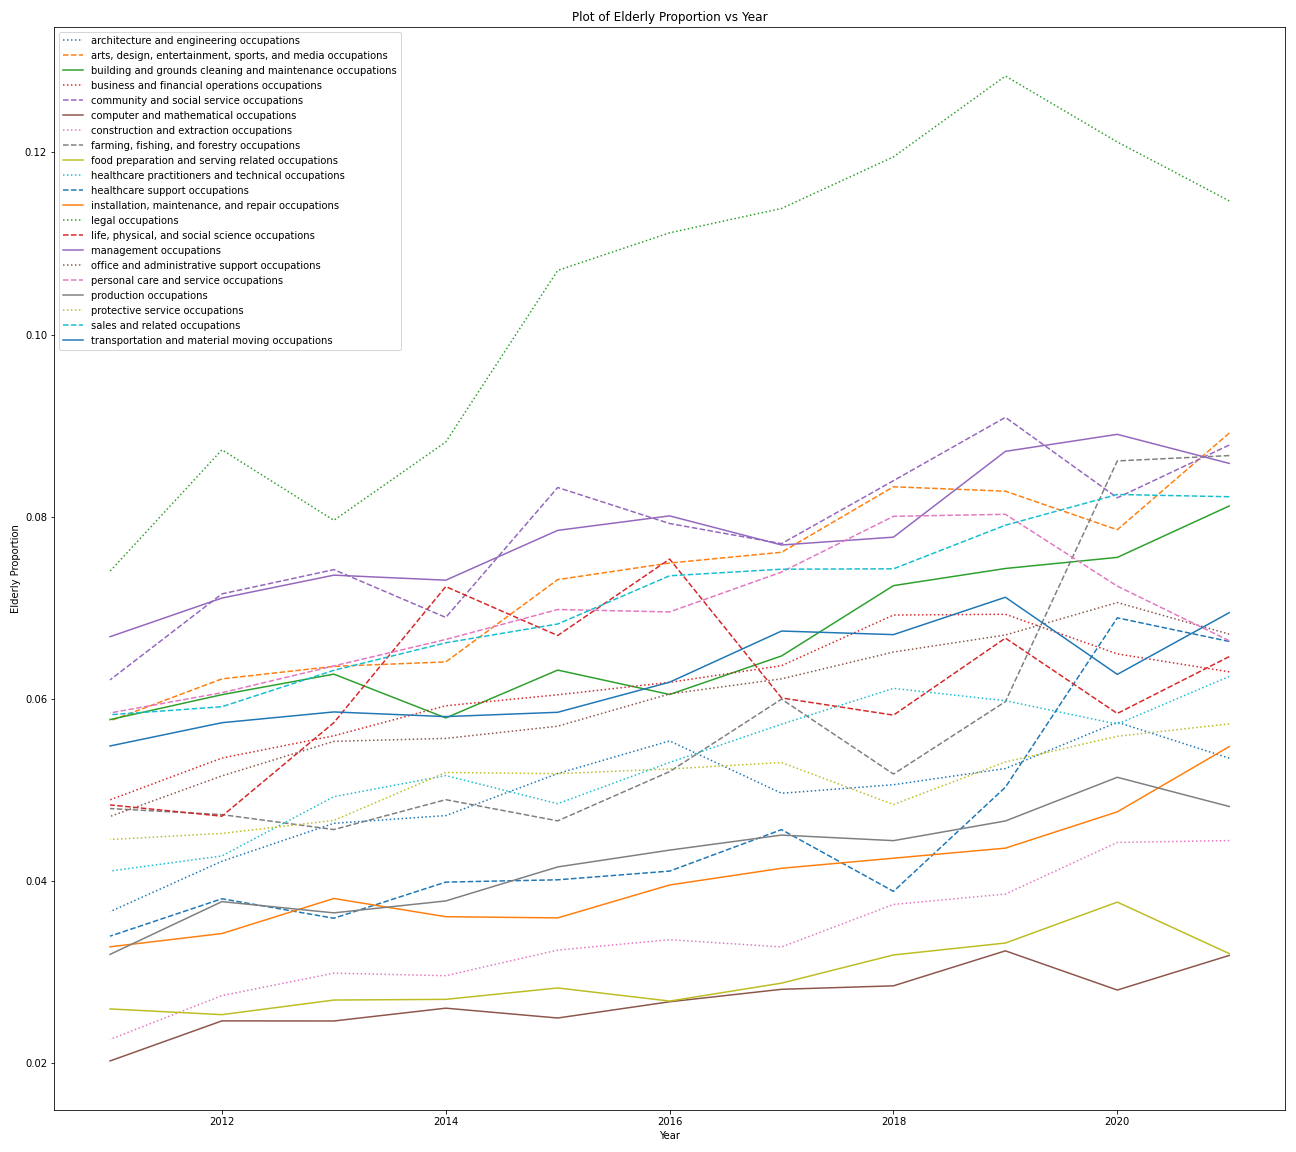
\includegraphics[width=12cm]{Figures/Elderly Proportion against Year}\label{fig:EP against year}}
	\hfill
	\subfloat[Old Proportion]{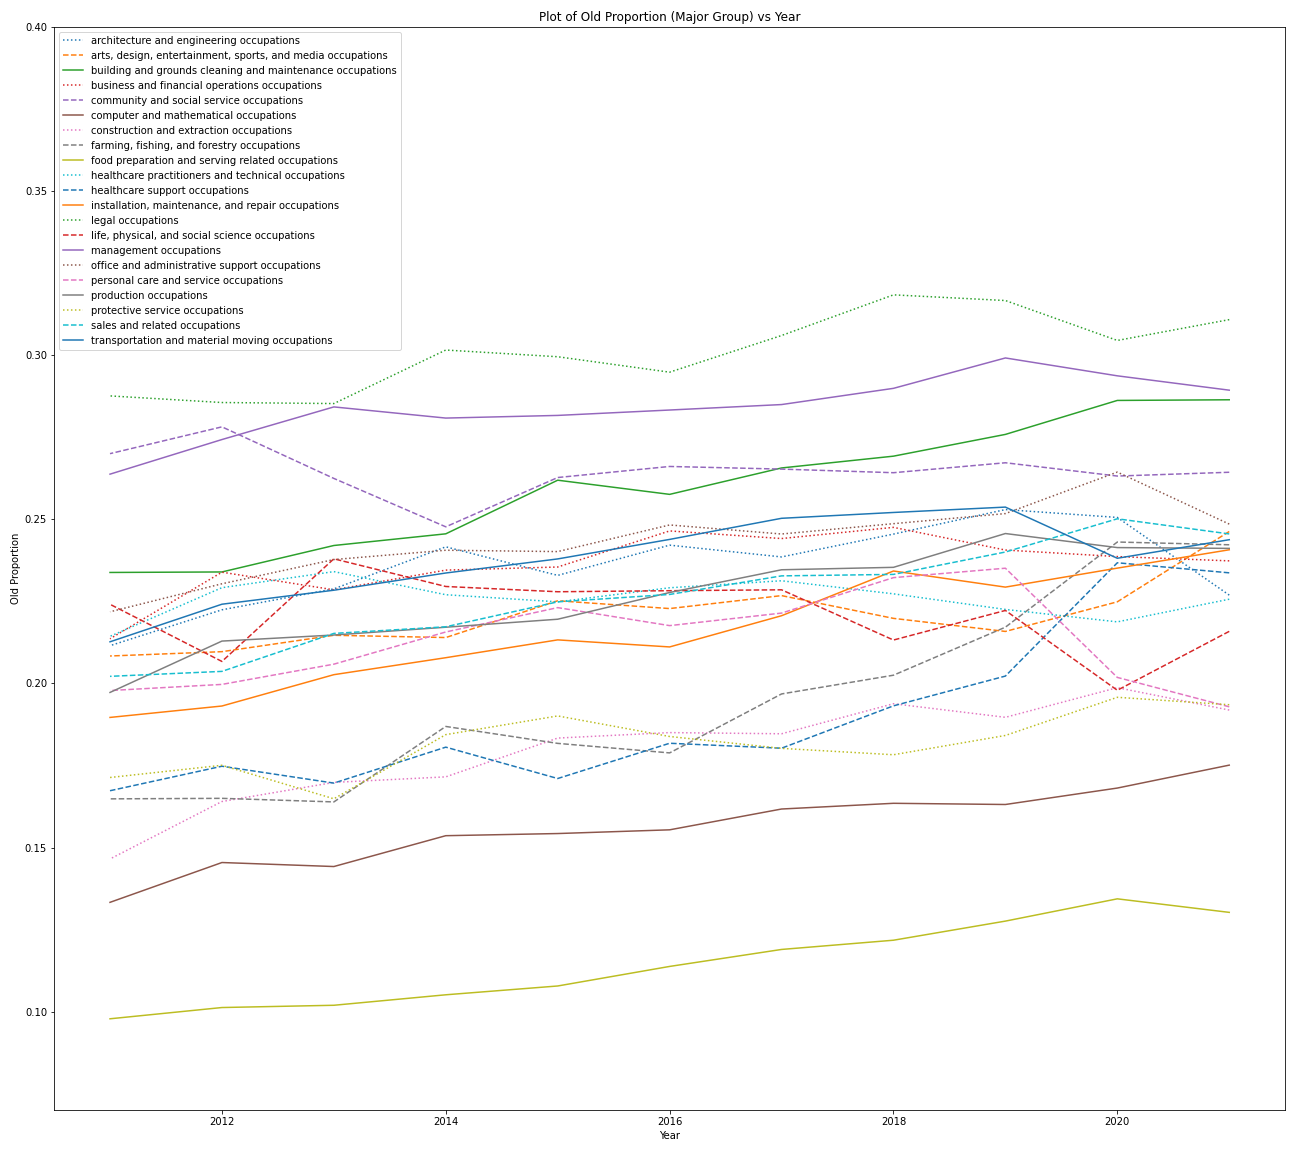
\includegraphics[width=12cm]{Figures/Old Proportion against Year}\label{fig:OP against year}}
	\hfill
	\caption{Plot of EP/OP (for each Major Groups) against Year. There is a general increase across most of the Major Group occupations, which is expected given the ageing population in the United States.}
	\label{fig:EP/OP against year}
\end{figure}

That being said, it is rather tricky to make sense of Figure \ref{fig:EP/OP against year} given that there are 21 individual plots within each of the two figures. Hence, we can calculate the relative change in EP/OP each Major Group occupation from 2011 to 2021 to obtain Figure \ref{fig:relativechange}. With regards to EP, the `construction and extraction occupations' had the highest relative increase while the `personal care and service occupations' had the least. When we look at OP, 'farming, fishing, and forestry occupations' had the highest relative increase, while there are some occupations that had a relative decrease. The 'life, physical, and social science occupations' had the largest relative decrease. However, this relative decrease is still merely about 4\%, so it is accurate to say that there is a general trend of ageing across the occupations.

These findings are not surprising given what was discussed in Chapter \ref{subsec:ageingpopulation}. We expect that an ageing population would lead to an ageing labour force. In fact, we can expect that these occupations will age even more over the next few decades.


\begin{figure}[!htb]
	\centering
	\subfloat[Elderly Proportion]{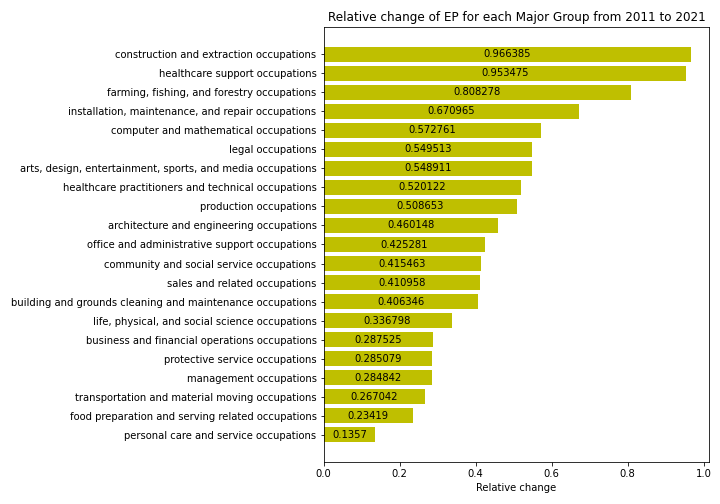
\includegraphics[width=13cm]{Figures/Relative change of EP.png}\label{fig:Relative change of EP}}
	\hfill
	\subfloat[Old Proportion]{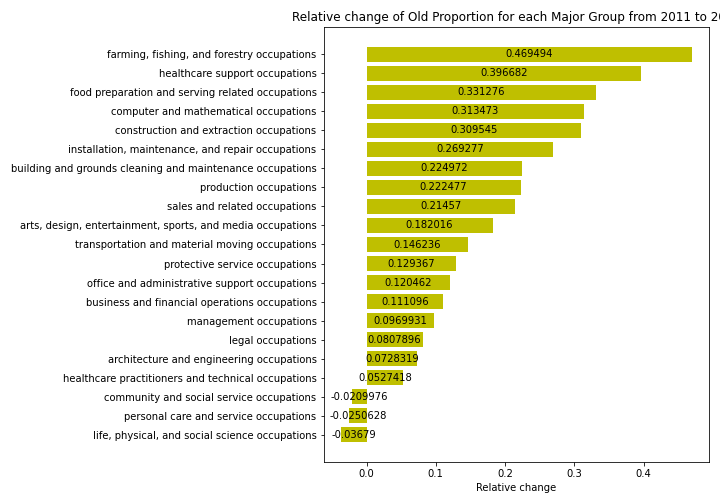
\includegraphics[width=13cm]{Figures/Relative change of OP}\label{fig:Relative change of OP}}
	\hfill
	\caption{Relative change of EP/OP for each Major Group from 2011 to 2021. This shows us which occupations experienced the most and least rapid ageing during the time period of 2011 to 2021.}
	\label{fig:relativechange}
\end{figure}


% \begin{figure}[!htb]
% 	\centering
% 	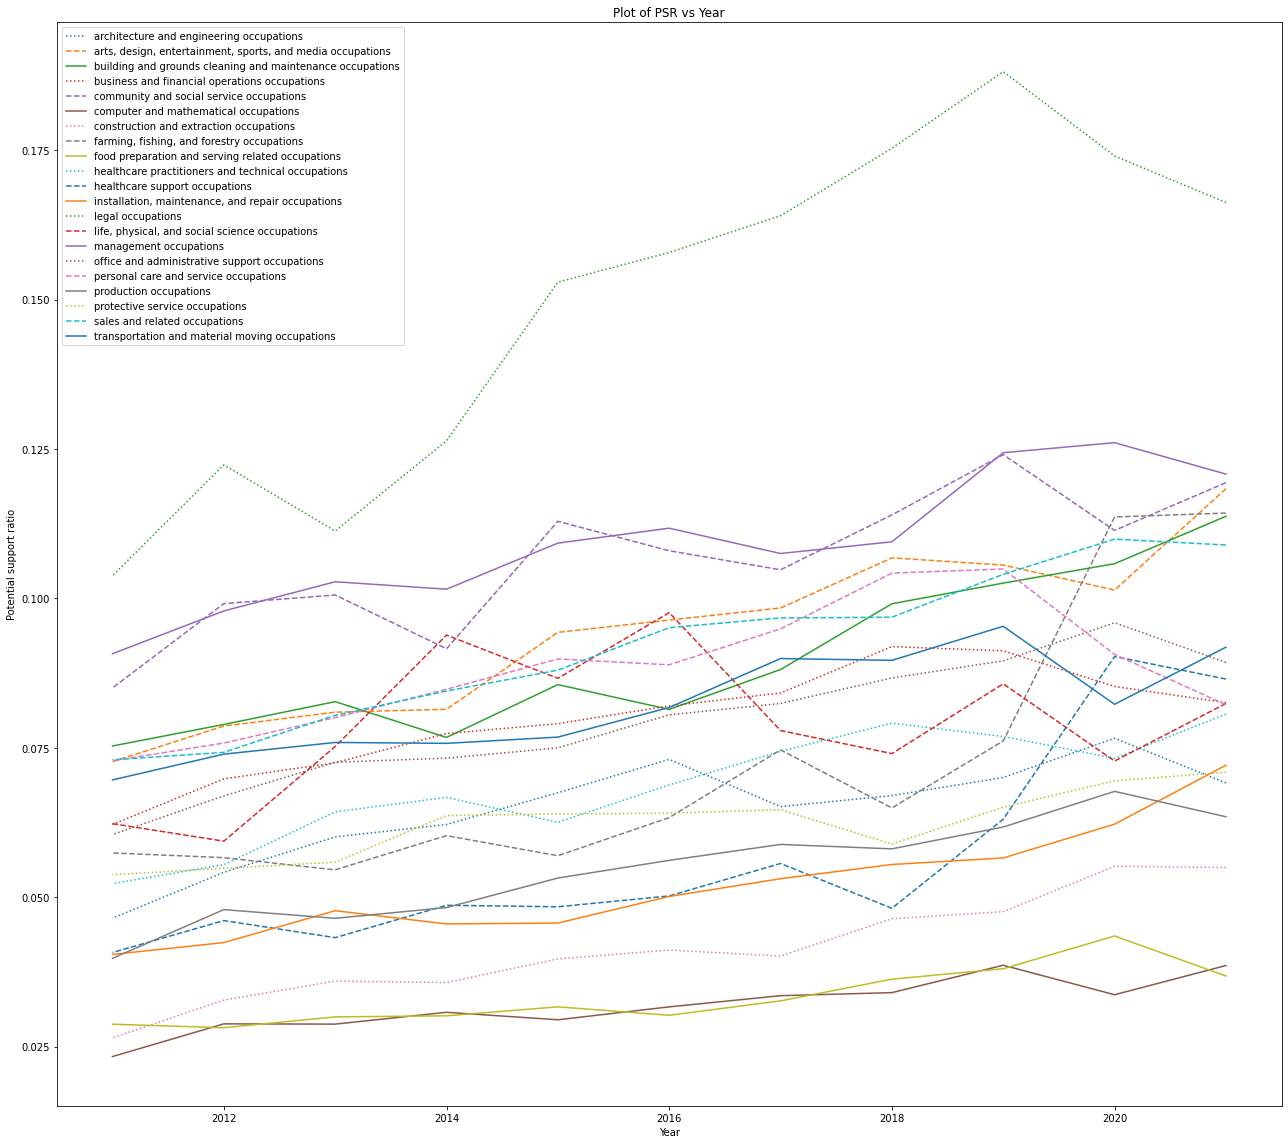
\includegraphics[width=17cm]{/Users/terencetan/Documents/Uni stuff/Engineering Science/4YP/4YP-The-Future-of-Work/Report/Figures/PSR vs Year.png}
% 	\caption{Plot of PSR vs Year for Major Groups}
% 	\label{fig:psrvsyear}
% \end{figure}

\clearpage

\section{Data Analysis}

Now that we have our processed BLS dataset (with the calculated OP and EP), we can use \emph{Pandas.merge} to join it with the automatability dataset (which includes the Probability of Computerisation) from \cite{futureofemployment} based on the Detailed Occupation. This gives us a joint data set that we will refer to as \emph{joint\_auto}. Unfortunately, the BLS dataset does not feature a full list of all the Detailed Occupations, so we end up with a reduced set of Detailed Occupations in the \emph{joint\_auto} dataset. As can be seen in Figure \ref{fig:jointautoratio}, \emph{joint\_auto} only represents about 40\% of the total US civilian labour force, which is still a significant amount. However, there is the question of whether \emph{joint\_auto} is a representative sample of the population, i.e. the US civilian labour force. We shall analyse this question by treating it as a population sampling problem.

\begin{figure}[!htb]
	\centering
	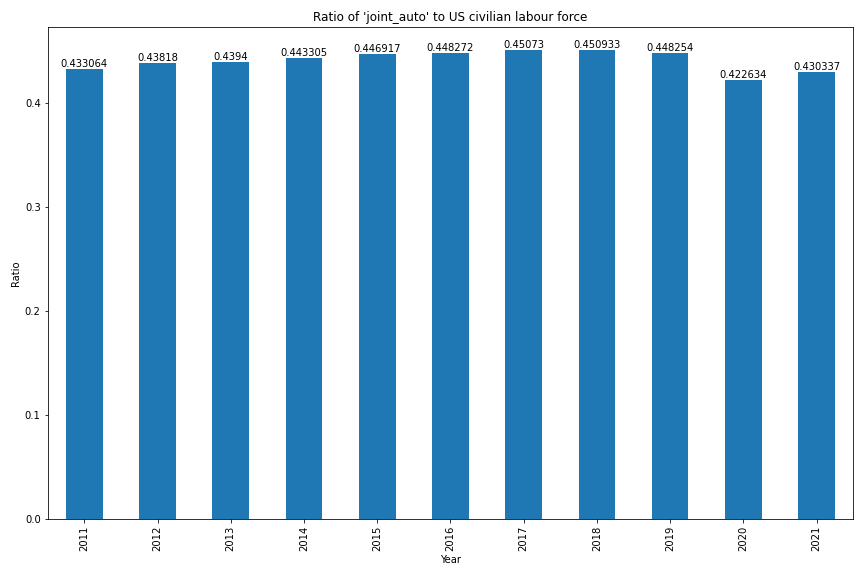
\includegraphics[width=12cm]{Figures/joint_auto ratio.png}
	\caption{Plot of ratio of \emph{joint\_auto} to US civilian labour force against Year. We can see that our \emph(joint\_auto) dataset represents a significant proportion of the total labour force, but not enough for us to generalise any trends we may find in our dataset. We will have to investigate how well our dataset represents the actual US civilian labour force.}
	\label{fig:jointautoratio}
\end{figure}


\subsection{Checking biasness}
\label{subsec:Checking biasness}
As mentioned earlier, we shall treat \emph{joint\_auto} as the sample and the US civilian labour force as the population. We shall use the Major Group occupations from our processed BLS dataset to represent the US civilian labour force since we have established its high representation in Chapter \ref{sec:prelim findings}.

We start off with a simple mean and variance comparison.  We find the mean and variance of the OP, EP, and PCom values for both the sample and population, which are shown in Table \ref{tab:mean and variance}. We can see that the means and variances match quite well for the PCom variable. For OP and EP, the means match quite closely, but the variances are off by an order of magnitude; the sample have a higher variance than the population for both OP and EP. This means that the sample have more spread-out values for OP and EP, so we must exercise caution when generalising any findings from the sample to the population. Otherwise, the sample seems fairly representative of the population. That being said, the mean and variance analysis is too simplistic to give us any concrete conclusions. Hence, we need a more sophisticated measure of the sample's representativeness of the population.

\begin{table}[]
	\centering
	\begin{tabular}{l|ll|ll}
					  & \multicolumn{2}{l|}{\textbf{Population}} & \multicolumn{2}{l}{\textbf{Sample}} \\ \cline{2-5} 
	\textbf{Variable} & Mean               & Variance            & Mean            & Variance          \\ \hline
	EP                & 0.0578             & 0.000394            & 0.0516          & 0.00334           \\ \hline
	OP                & 0.220              & 0.00190             & 0.223           & 0.0122            \\ \hline
	PCom              & 0.536              & 0.136               & 0.508           & 0.143            
	\end{tabular}
	\caption{Population/Sample mean and variance. We can see that the means and variances are very similar between the sample and the population. However, we note that the EP/OP values for the sample have higher variances compared to that of the population.}
	\label{tab:mean and variance}
\end{table}


We can look at the proportion of the total number of people employed within each Major Group with respect to the total US civilian labour force for each year. For example, Management Occupations represent 13.2\% of the US civilian labour force in 2021, 13.4\% in 2020 and so on. Transportation and Material Moving Occupations represent 6.34\% in 2011, 6.38\% in 2012 and so on. We put all of this information into one vector, which would represent the population proportion. We then map all the occupations (which are Detailed Occupations) in \emph{joint\_auto} back to their respective Major Groups, and sum up the number of people employed in each of those Detailed Occupations within the Major Groups for each year. These numbers are then divided by the total number of people employed in \emph{joint\_auto} for each year. This would tell us the proportion of each of the 21 Major Groups within \emph{joint\_auto} for each year; this sample proportion information would be placed in another vector. We want to see how well the sample proportion vector matches the population proportion vector, so we subtract the former from the latter and plot the result in Figure \ref{fig:relativeweightage}. We can see that the values along the y-axis are all fairly small. Just to illustrate this point further, we plot the sample proportion against the population proportion in Figure \ref{fig:sampleprop vs popprop}. Ideally, we would like the plot to be a straight line with a gradient of 1 and a y-intercept of 0, and we can see that our plot does closely resemble such a line. Indeed, fitting a best-fit line to the plot confirms this as well, with the best-fit line having a gradient of 1.18 and a y-intercept of -0.00862. Hence, the sample has a similar makeup to the population in terms of the relative weightage of each of the Major Groups.

Given our above biasness tests, we can make the reasonable assumption that our sample is fairly representative of the population, and any findings obtained from the sample can be generalised to the population to a certain extent.


\begin{figure}[!htb]
	\centering
	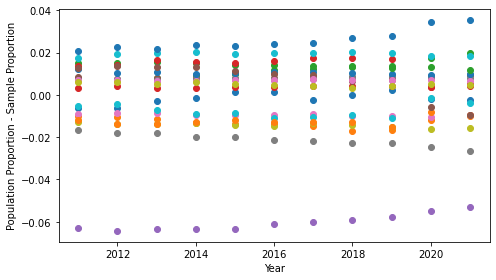
\includegraphics[width=12cm]{Figures/sample test.png}
	\caption{Plot of the difference between the population proportion and the sample proportion against Year. The different colours represent different Major Groups. The low values along the y-axis shows that the relative weightage of each of the Major Groups within the sample is similar to that of the population. Hence, the sample has a similar makeup to the population in terms of the Major Groups.}
	\label{fig:relativeweightage}
\end{figure}

\begin{figure}[!htb]
	\centering
	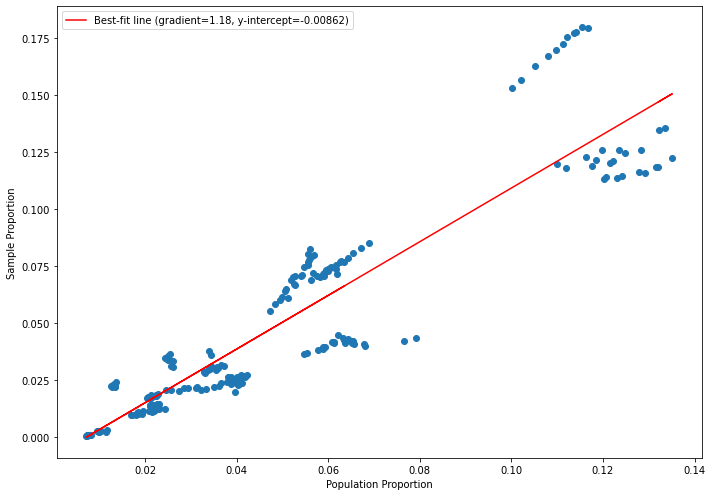
\includegraphics[width=12cm]{Figures/Sample Proportion against Population Proportion.png}
	\caption{Plot of the sample proportion against population proportion (with a best-fit line). We can see that our plot roughly follows a straight line with a gradient of 1 and y-intercept of 0.}
	\label{fig:sampleprop vs popprop}
\end{figure}

\subsection{Exploration of Data}
Now that we have established the representativeness of the sample, we can go about exploring the dataset. 

\subsubsection*{EP/OP against PCom}

The first thing we do is to create a scatterplot of the Detailed Occupations within \emph{joint\_auto}, with the EP/OP values (for 2012 only since the PCom values were calculated based on 2012 data) on the y-axis and the PCom values on the x-axis. We also scale each data point relative to the total number of people employed within that occupation, i.e. occupations with more people will be bigger on the plot. This gives us Figure \ref{fig:EP/OP against PCom}, which we can see has no obvious trends. Zooming in on specific regions of the scatterplot (e.g. the region of high PCom) also yields no significant patterns. We also calculated the correlation coefficients, which can be found in Table \ref{tab:correlation}. We do note that the majority of employed workers are concentrated in either the low PCom region or the high PCom region, with relatively few in between. This is consistent with the findings from \cite{osborne2017future}, and is another piece of evidence that our assumption that \emph{joint\_auto} is fairly representative of the US civilian labour force is reasonable as discussed in Chapter \ref{subsec:Checking biasness}. 

\begin{figure}[!htb]
	\centering
	\subfloat[Elderly Proportion]{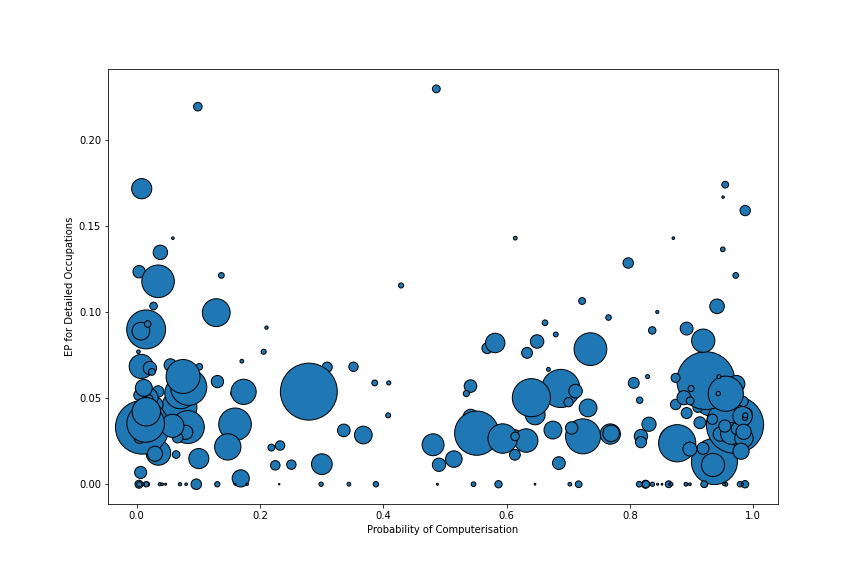
\includegraphics[width=15cm]{Figures/Scatterplot of EP for DO}\label{fig:EP against PCom}}
	\hfill
	\subfloat[Old Proportion]{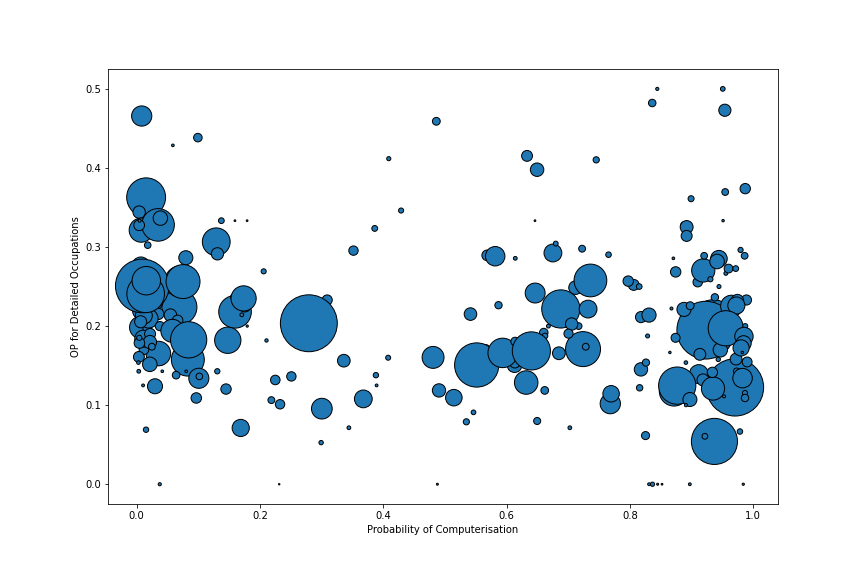
\includegraphics[width=15cm]{Figures/Scatterplot of OP for DO}\label{fig:OP against PCom}}
	\hfill
	\caption{Plot of EP/OP (for each Detailed Occupation) against PCom. There seems to be no obvious patterns or trends present.}
	\label{fig:EP/OP against PCom}
\end{figure}

\begin{table}[]
	\centering
	\begin{tabular}{l|ll|ll}
	\textbf{Type of correlation} & \multicolumn{2}{l|}{\textbf{EP}} & \multicolumn{2}{l}{\textbf{OP}} \\ \hline
	Pearson                      & \multicolumn{2}{l|}{-0.00363}     & \multicolumn{2}{l}{-0.0321}      \\ \hline
	Spearman                     & \multicolumn{2}{l|}{-0.0151}      & \multicolumn{2}{l}{-0.0661}    \\ \hline
	Kendall                      & \multicolumn{2}{l|}{-0.00881}      & \multicolumn{2}{l}{-0.0429}   
	\end{tabular}
	\caption{Correlation coefficients for Figure \ref{fig:EP/OP against PCom}}
	\label{tab:correlation}
	\end{table}


Our next step of exploration is to take the base 10 logarithmic\footnote{as can be seen in Figure \ref{fig:EP/OP against PCom}, the occupations with zero values for EP/OP have relatively few people employed within them, and we can remove them beforehand to avoid negative infinite values without affecting the representativeness of our dataset too much} of EP/OP and PCom, and plot the former against the latter in a scatterplot, as shown in Figure \ref{fig:logEP/OP against PCom}. Interestingly, the $\log_{10}$(OP) plot in Figure \ref{fig:logOP against PCom} seems to show a slight downward trend as $\log_{10}$(PCom) increases; plotting the scatterplot on a logarithmic scale seems to have revealed a previously hard-to-spot trend. We also calculated the correlation coefficients for this particular plot (along with the corresponding plot for EP), which is given in Table \ref{tab:logcorrelation}. This trend suggests that 'older' occupations tend to be less likely to be computerised. This makes intuitive sense for occupations such as management; \cite{osborne2017future} notes that management occupations tend to be at low risk of computerisation due to the high degree of social intelligence required for them, and people in management positions would also tend to be older since such occupations (especially the ones like Chief Executive Officer) would be biased towards those with more work experience. There is also some evidence that high skilled workers, who would generally be less likely to have their jobs computerised, tend to retire later than low skilled workers (\cite{HimmelreicherRalfK.2009Saao}).


\begin{table}[]
	\centering
	\begin{tabular}{l|ll|ll}
	\textbf{Type of correlation} & \multicolumn{2}{l|}{\textbf{EP}} & \multicolumn{2}{l}{\textbf{OP}} \\ \hline
	Pearson                      & \multicolumn{2}{l|}{0.00579}     & \multicolumn{2}{l}{-0.113}      \\ \hline
	Spearman                     & \multicolumn{2}{l|}{-0.0151}      & \multicolumn{2}{l}{-0.0661}    \\ \hline
	Kendall                      & \multicolumn{2}{l|}{-0.00881}      & \multicolumn{2}{l}{-0.0429}   
	\end{tabular}
	\caption{Correlation coefficients for Figure \ref{fig:logEP/OP against PCom}}
	\label{tab:logcorrelation}
	\end{table}


\begin{figure}[!htb]
	\centering
	\subfloat[Elderly Proportion]{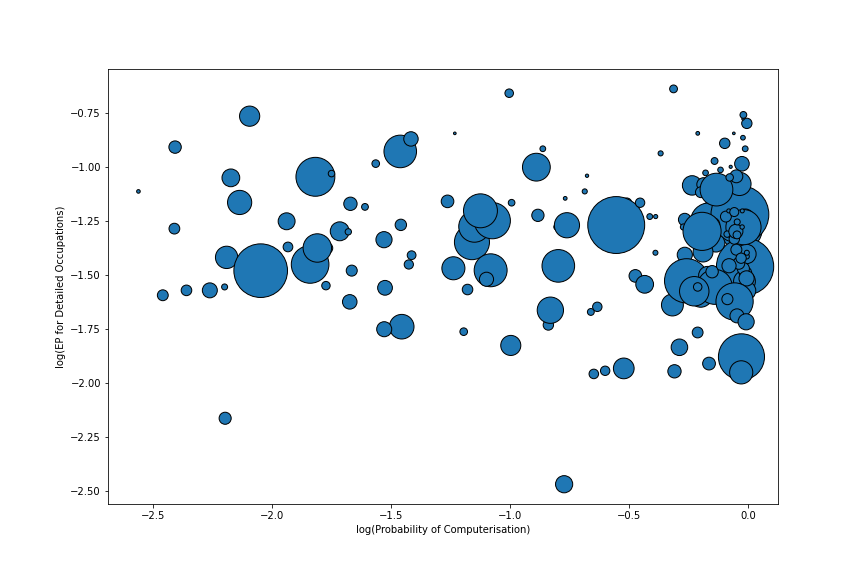
\includegraphics[width=15cm]{Figures/Scatterplot of log(EP) for DO}\label{fig:logEP against PCom}}
	\hfill
	\subfloat[Old Proportion]{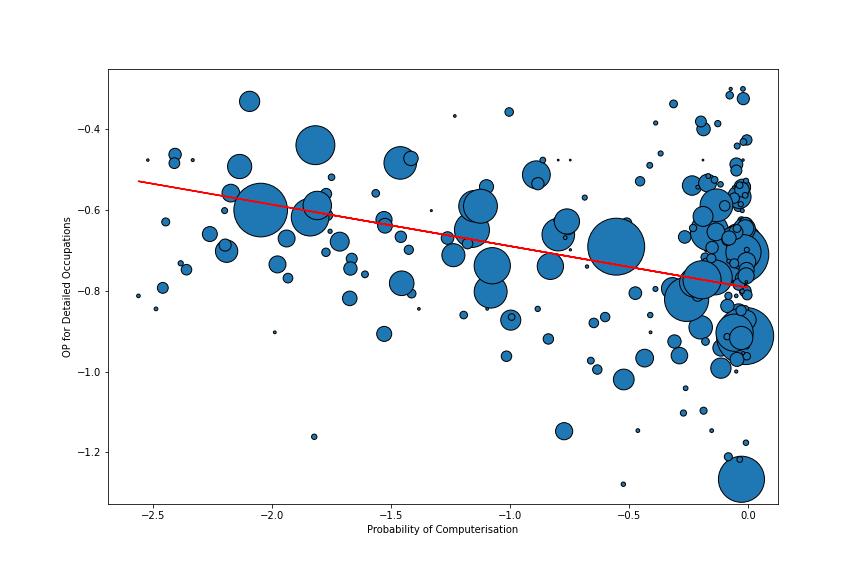
\includegraphics[width=15cm]{Figures/Scatterplot of log(OP) for DO}\label{fig:logOP against PCom}}
	\hfill
	\caption{Plot of $\log_{10}$(EP)/$\log_{10}$(OP) (for each Detailed Occupation) against $\log_{10}$(PCom). There seems to be a slight downward trend for the $\log_{10}$(OP) plot. This suggests that occupations that are less susceptible to computerisation tend to have a higher proportion of old people.}
	\label{fig:logEP/OP against PCom}
\end{figure}


Plotting the dataset grouped by Category Labels or Major Groups do not seem to yield any interesting results either. In fact, there are too few datapoints for some of the Labels and Major Groups for us to draw any meaningful conclusions.

\subsubsection*{Relative change of EP/OP against PCom}
In the previous section, we plotted EP/OP values for 2012 against PCom on a scatterplot. It seems like a waste to not use more of the EP/OP values for the other years given all our efforts to clean the dataset in Chapter \ref{sec:Dataset}. We can use the EP/OP values for 2011 and 2021 to calculate the relative change of EP/OP for the Detailed Occupations from 2011 to 2021, similar to what we did in Figure \ref{fig:relativechange}. Plotting the relative change values against PCom in a scatter plot gives us Figure \ref{fig:Relative change against PCom}. We also calculated the correlation coefficients, which can be found in Table \ref{tab:correlation for relative}. Although there seems to be no obvious trends in Figure \ref{fig:Relative change against PCom}, the Pearson correlation coefficient for the relative change of OP with PCom is relatively high.

Due to the fact that the relative change of EP/OP could be negative, taking the logarithmic would prove to be tricky. It is hard to justify simply removing negative values from the dataset because we would be ignoring all occupations which became 'younger' from 2011 to 2021 and they are an essential part of the dataset. Hence, we will not plot a logarithmic scale scatterplot as we had done in the previous section.


\begin{figure}[!htb]
	\centering
	\subfloat[Elderly Proportion]{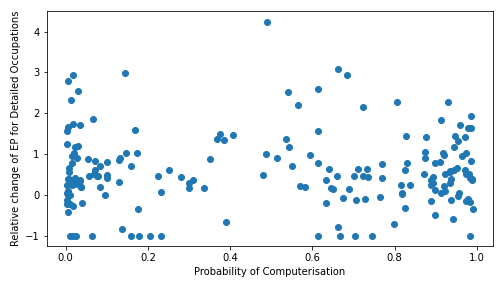
\includegraphics[width=15cm]{Figures/Scatter Relative change of EP for DO.png}\label{fig:relativeEP against PCom}}
	\hfill
	\subfloat[Old Proportion]{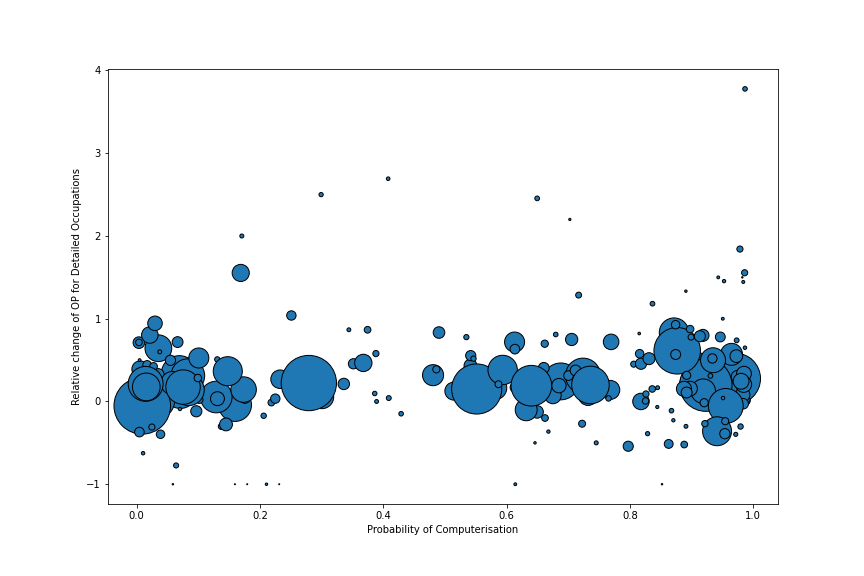
\includegraphics[width=15cm]{Figures/Scatter Relative change of OP for DO.png}\label{fig:relativeOP against PCom}}
	\hfill
	\caption{Plot of relative change of EP/OP from 2011 to 2021 (for each Detailed Occupation) against PCom. There does not appear to be any noticeable trends.}
	\label{fig:Relative change against PCom}
\end{figure}

\begin{table}[]
	\centering
	\begin{tabular}{l|ll|ll}
	\textbf{Type of correlation} & \multicolumn{2}{l|}{\textbf{EP}} & \multicolumn{2}{l}{\textbf{OP}} \\ \hline
	Pearson                      & \multicolumn{2}{l|}{0.0143}     & \multicolumn{2}{l}{0.180}      \\ \hline
	Spearman                     & \multicolumn{2}{l|}{0.0247}      & \multicolumn{2}{l}{0.190}    \\ \hline
	Kendall                      & \multicolumn{2}{l|}{0.0191}      & \multicolumn{2}{l}{0.128}   
	\end{tabular}
	\caption{Correlation coefficients for Figure \ref{fig:Relative change against PCom}}
	\label{tab:correlation for relative}
	\end{table}

\subsection{Conclusion}
We did not find any strong trends despite using different metrics and plot scales. The most interesting results arose from the OP values, specifically the relationships of $\log_{10}$(OP) and relative change of OP with respect to $\log_{10}$(PCom) and PCom respectively. The latter has a particularly high (relative to the others) Pearson correlation coefficient, while the former has a more obvious trend in the scatterplot. We should note that the each datapoint in the scatterplots had its size scaled relative to the number of people employed within that particular occupation. On the other hand, our correlation coefficients were calculated without regard for this scaling. Hence, it might be worth investigating the weighted correlation coefficients. Given that both of the interesting relationships seem to be somewhat linear in nature, we shall focus on the weighted Pearson correlation. To calculate the weighted Pearson correlation between two vectors $x$ and $y$ with weight vector $w$ (all three vectors must have the same dimensions), we can use the following equations (\cite{bailey2018weighted}):

\begin{equation} \label{eq1}
	\begin{split}
		\text{Weighted mean}: m(x; w) & = \frac{\sum_{i}w_{i}x_{i}}{\sum_{i}w_{i}}. \\
		\text{Weighted covariance}: cov(x, y; w) & = \frac{\sum_{i}w_{i}(x_{i}-m(x; w))(y_{i}-m(y; w))}{\sum_{i}w_{i}}. \\
		\text{Weighted correlation}: corr(x, y; w) & = \frac{cov(x, y; w)}{\sqrt{cov(x, x; w)cov(y, y; w)}}.
	\end{split}
	\end{equation}

Applying these equations on our data would give us the values in Table \ref{tab:weightedpearson}. The weighted correlation for $\log_{10}$(OP) and $\log_{10}$(PCom) is much larger (in absolute terms) than the unweighted correlation, and better matches what we see in Figure \ref{fig:logOP against PCom}. It's absolute value is also larger than the weighted correlation for relative change of OP and PCom.


\begin{table}[]
	\centering
	\begin{tabular}{l|l}
	\textbf{Variables}                                              & \textbf{Weighted Pearson Correlation} \\ \hline
	\begin{tabular}[c]{@{}l@{}}Relative change of OP\\ vs\\ PCom\end{tabular} & 0.198                                 \\ \hline
	\begin{tabular}[c]{@{}l@{}}$\log_{10}$(OP)\\ vs\\ $\log_{10}$(PCom)\end{tabular}               & -0.434                              
	\end{tabular}
	\caption{Weighted Pearson Correlation showing that the strongest trend we have found so far is the relationship between the $\log_{10}$(OP) for 2012 and $\log_{10}$(PCom).}
	\label{tab:weightedpearson}
	\end{table}

Hence, the strongest trend so far is the relationship between OP and PCom. In addition, it appears to be a somewhat linear trend. Hence, we will be focus on applying linear regression to this set of variables in the next section.


\subsection{Linear Regression}
\label{subsec:Linear Regression}
In this section, we will be applying a number of linear regression techniques (using the Scikit\-learn package\footnote{https://scikit-learn.org} for Python) on the OP and PCom values, specifically weighted least squares, weighted Bayesian ridge, weighted Huber, and RANdom SAmple Consensus (RANSAC). We use take the weights into account for most of the models since we got the highest correlation when weights were taken into account. All of the mentioned techniques can be applied on the other data values; we only picked the $\log_{10}$(OP) vs $\log_{10}$(PCom) relationship because that is the one that displayed the strongest trend so far. Another caveat is that this particular trend is not that strong, and further analysis should be conducted to determine whether it is actually statistically significant. We will further elaborate on this point in the \textbf{FUTURE WORK SECTION}.

In a least squares model, the dependent variable is a linear combination of the independent variables along with an error term:

\begin{equation}
	\label{eq:LS}
    y_{i}=x^{T}_{i}\beta + \epsilon_{i} \quad \textrm{for} \quad i=1,...,m,
\end{equation}
where $m$ is the number of samples, $y_{i}$ is the $i^{th}$ observation of the dependent variable, $x^{T}_{i}$ is the corresponding row vector of all the independent variables, and $\epsilon_{i}$ is the corresponding error term. In our case, $x_{i}$ and $\beta$ are both just $2\times1$ vectors since we only have the one independent variable PCom (the second element of the vectors corresponds to the y-intercept of the linear model). We also define the vector and matrix $y = [y_{1},...,y_{m}]^{T}$ and $X^{T} = [x_{1},...,x_{m}]$ respectively.


\subsubsection*{Weighted Least Squares}

In a weighted least squares model, we aim to minimise (with respect to $\beta$) the following function:

\begin{equation}
	\label{eq:WLS}
    S=\sum^{m}_{i=1} w_{i}(y_{i}-x^{T}_{i}\beta)^{2},
\end{equation}

where $w_{i}$ is the corresponding $i^{th}$ scalar weight.

Doing so gives us the plot in Figure \ref{fig:WLS}, which we can see fits the downward trend fairly well. Note that ordinary least squares is a special case of weighted least squares with all weights being equal to unity.

\subsubsection*{Bayesian Ridge}
For a Bayesian approach, we implement linear regression using probability distributions rather than point estimates like with the weighted least squares method. We model our observation $y$ as follows:

\begin{equation}
	\label{eq:likelihood}
    \mathcal{P}(y | \beta, X, \alpha) = \mathcal{N}(y | X\beta, \alpha),
\end{equation}

where $\alpha$ is a hyper parameter.

We also model the prior for the coefficients $\beta$ as follows:

\begin{equation}
	\label{eq:prior}
    \mathcal{P}(\beta | \lambda) = \mathcal{N}(\beta | 0, \lambda^{-1}I),
\end{equation}

where $\lambda$ is another hyper parameter and $I$ is a $2\times2$ identity matrix.

Additionally, we model the priors for $\alpha$ and $\lambda$ as gamma distributions. We then write out the posterior distribution as follows:

\begin{equation}
	\label{eq:posterior}
    \mathcal{P}(\beta | y,X,\lambda,\alpha) = \frac{\mathcal{P}(y | \beta, X, \lambda, \alpha)\mathcal{P}(\beta | X, \lambda, \alpha)}{\mathcal{P}y | X, \lambda, \alpha)}.
\end{equation}

The hyper parameters $\alpha$ and $\lambda$ are estimated by maximising the log marginal likelihood (method for doing so is described in \cite{tipping2001sparse}). Using these estimates and the above probability distributions, we can obtain an estimate for $\beta$ by taking the mean of the posterior distribution in Equation \ref{eq:posterior}. Note that the Scikit\-learn implementation\footnote{https://github.com/scikit-learn/scikit-learn/blob/9aaed4987/sklearn/linear\_model/\_bayes.py} of Bayesian Ridge involves an iterative process of updating the posterior mean and calculating the corresponding the root mean square error between the predicted values of $y$ and the actual values of $y$, and then updating the estimates of the hyper parameters $\alpha$ and $\lambda$ using the calculated root mean square error. The weights of each datapoint is taken into account in this implementation by scaling each datapoint $(x_{i}, y_{i})$ by the square root of the corresponding weight $w_{i}$ to get $(scaled\_x_{i}, scaled\_y_{i}) = (\sqrt{w_{i}} x_{i}, \sqrt{w_{i}} y_{i})$ \footnote{Calculating the root mean square error with this scaling is equivalent to using the weighted root mean square $S$ defined in Equation \ref{eq:WLS}.}. By doing so, datapoints with a higher weight will contribute more to the root mean square error, thereby having a bigger effect on the update of the hyper parameters and consequently the update of the posterior mean.

%$$\displaystyle{\displaylines{\sqrt{w_{i}}x_{i}}}$$

\subsubsection*{RANdom SAmple Consensus (RANSAC)}
Unlike the previous two regression models, RANSAC models attempt to identify the inliers and outliers, and then completely ignore the outliers.

The RANSAC algorithm has two main steps. Firstly, a subset of the datapoints are randomly chosen to construct a model along with the model parameters. Secondly, the algorithm then tests all datapoints against this model. Datapoints which exceed a certain error threshold would be labelled as outliers while the rest would be inliers. These two steps are then repeated until the number of inliers exceed a certain selected threshold. In our case, the model constructed is restricted to a linear model, and the error is calculated using Equation \ref{eq:WLS} (thereby allowing us to incorporate the weights into the training process of the model).

Applying RANSAC on our datapoints give us Figure \ref{fig:RANSAC}. We can see that the algorithm correctly identifies the outliers and give a regression line that is very similar to the ones predicted by weighted least square and Bayesian ridge.

\begin{figure}[!htb]
	\centering
	\subfloat[Weighted least squares (gradient: -0.103, y-intercept: -0.793)]{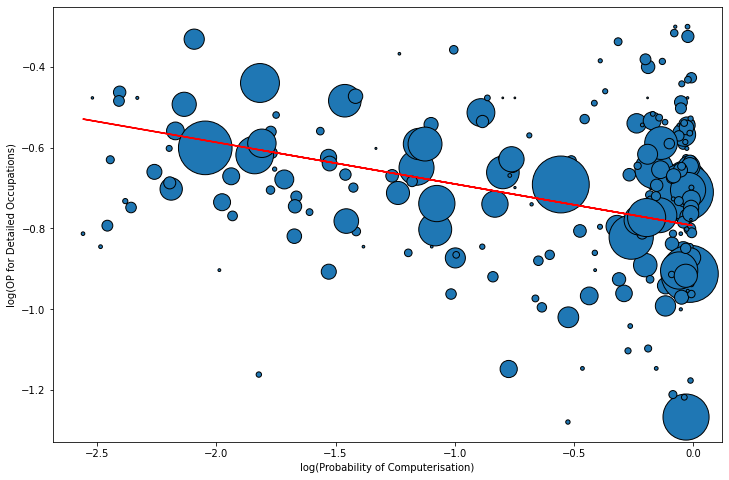
\includegraphics[width=11cm]{Figures/Weighted Least Squares.png}\label{fig:WLS}}
	\hfill
	\subfloat[Bayesian ridge (gradient: -0.101, y-intercept: -0.791)]{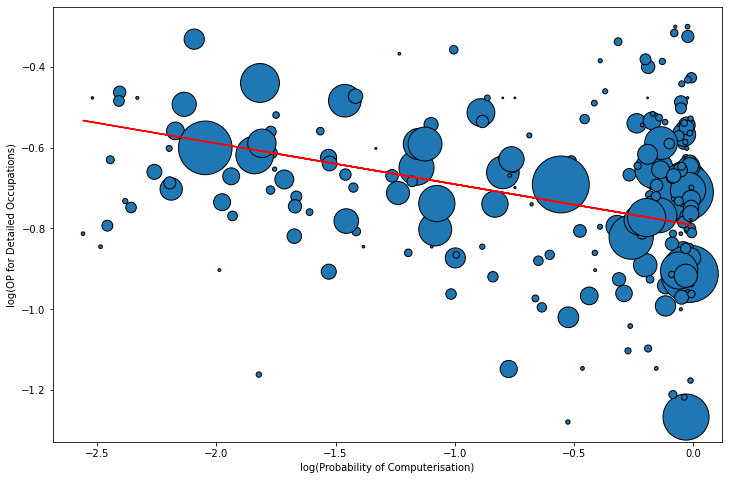
\includegraphics[width=11cm]{Figures/Bayesian ridge}\label{fig:bayesian ridge}}
	\hfill
 	\subfloat[RANSAC (gradient: -0.110, y-intercept: -0.782]{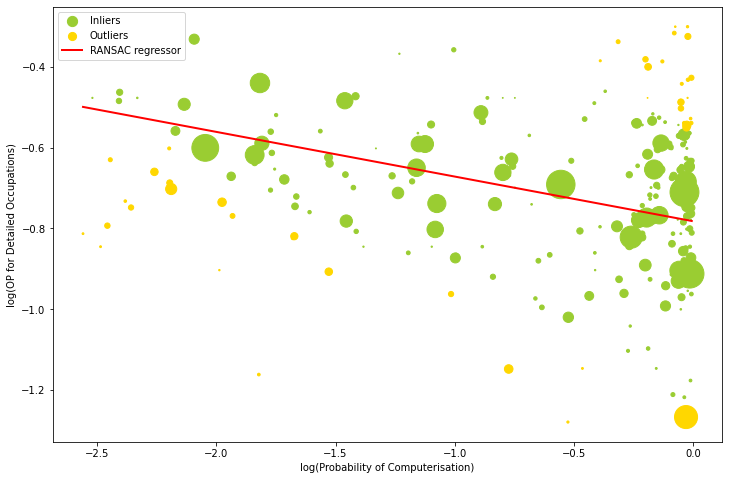
\includegraphics[width=11cm]{Figures/RANSAC.png}\label{fig:RANSAC}}
	\hfill
	\caption{Plot of $\log_{10}$(OP) against $\log_{10}$(PCom). The red lines represent the respective linear regressors.}
	\label{fig:RANSAC}
\end{figure}




\subsubsection*{Conclusion}
Having tried various linear regression methods, we obtain very similar results for all of them. These results could be used to predict the OP values of the occupations missing from our \emph{joint\_auto} dataset. However, we note that there is a high level of variance around our linear regression lines. Hence, any predicted values we get might not be that useful. Instead, it might be better if we could define a minimum region which contains most if not all of our known datapoints, and has a low chance of not encompassing any unknown datapoints. We would ideally also like to quantify our confidence in such a region. We shall explore this idea in the next section.


\subsection{Probably Approximately Correct (PAC) Learning}
\label{subsec:PAC}
Suppose we have an unknown target set \emph{T} from which we obtained independent and identically distributed (i.i.d.) samples $\delta_{1},...,\delta_{m}$. Using the \emph{m} samples, we want to construct a hypothesis set $H_{m}$ that approximates \emph{T}. The framework we use to learn $H_{m}$ is known as PAC Learning.

Of course, we want $H_{m}$ to approximate \emph{T} as close as possible, such that the probability of a new sample $\delta$ from \emph{T} not belonging in $H_{m}$ is less than or equal to an arbitrary threshold probability $\epsilon$, i.e. $\mathbb{P}(\delta \in \emph{T} \setminus H_{m}) \leq \epsilon$. Since $H_{m}$ depends on the set of i.d.d. random samples $S = \{\delta_{1},...,\delta_{m}\}$, it is also random. This means that $\mathbb{P}(\delta \in \emph{T} \setminus H_{m}) \leq \epsilon$ is itself a random variable, allowing us to quantify a confidence for it:
\begin{equation}
	\label{eq:1}
	\mathbb{P}^{m} \{\delta_{1},...,\delta_{m}: \mathbb{P}(\delta \in \emph{T} \setminus H_{m}) \leq \epsilon \} \geq 1 - q(m,\epsilon),
\end{equation}
where $1 - q(m,\epsilon)$ is a lower bound to our confidence that the probability of a new sample not belong in $H_{m}$ is less than or equal to $\epsilon$. We refer the reader to (\cite{paclearning1}) for a more comprehensive introduction to this concept. In fact, this entire section on PAC Learning is heavily based on the work done by (\cite{paclearning1}), (\cite{romao2021tight}), and (\cite{kostas}).

Furthermore, consider the following convex scenario program:
\begin{equation}
	\label{eq:2}
	\begin{array}{rrclcl}
	\displaystyle \min_{x \in \mathbb{R}^{n_{x}}} & \multicolumn{3}{l}{c^{T}x}\\
	\textrm{s.t.} & g(x,\delta_{i}) \leq 0, \quad \textrm{for all i = 1,...,m}.\\
	\end{array}
	\end{equation}
Suppose $\delta_{i}$ belongs to an uncertainty space $\Delta$, i.e. $\delta_{i} \in \Delta$ for $i = 1,...,m$, and we have obtained the optimal solution $x^{*}_{m}$ to the scenario program in Equation \ref{eq:2}. If we then want to find out if a new $\delta\in \Delta$ will violate the constraint $g(x^{*},\delta) \leq 0$, we can use Equation \ref{eq:1} to quantify the probability of such a constraint violation happening. Let $T=\Delta$, $H_{m} = (\delta \in \Delta: g(x^{*}_{m},\delta) \leq 0)$, i.e. the set of samples for which $x^{*}_{m}$ remains feasible, and we get the following:

\begin{equation}
	\label{eq:3}
	\mathbb{P}^{m} \{\delta_{1},...,\delta_{m}: \mathbb{P}(\delta \in \Delta: g(x^{*}_{m},\delta) > 0) \leq \epsilon \} \geq 1 - q(m,\epsilon),
\end{equation}
where $\mathbb{P}(\delta \in \Delta: g(x^{*}_{m},\delta) > 0)$ is the probability that a new sample $\delta\in \Delta$ violates the constraint $(g(x^{*}_{m},\delta) \leq 0)$. Similar to Equation \ref{eq:1}, the probability of such a constraint violation should ideally to less than or equal to an arbitrary value $\epsilon$, and our confidence of that happening is at least $1 - q(m,\epsilon)$. Note that we did not specify a probability distribution for $T=\Delta$. This means that PAC Learning is a distribution-free technique, and we do not need to make any prior assumptions about the distribution of $\Delta$.

Before further elaborating on the $q(m,\epsilon)$ function, we want to first establish a few definitions.


\begin{theorem}
	A constraint is considered a support constraint if its removal changes the optimiser $x^{*}_{m}$. The support set of $x^{*}_{m}$, denoted by supp($x^{*}_{m}$), is the collection of support constraints for $x^{*}_{m}$.
\end{theorem}

\begin{theorem}
	We say that the convex scenario program \ref{eq:2} is fully-supported if, for any $S$ with $\abs{S} = m$ and $m > n_{x}$, $\abs{\text{supp}(x^{*}_{m})} = n_{x}$.
\end{theorem}

\begin{theorem}
	We say that the convex scenario program \ref{eq:2} is non-degenerate if, solving the program with only the support constraints in the support set supp($x^{*}_{m}$) gives us the same optimiser $x^{*}_{m}$ as when solving the program with all constraints (constructed with all the samples in $S$).
\end{theorem}

Note that if a problem is fully-supported, it is non-degenerate, but the converse does not hold.

Assuming $x^{*}_{m}$ exists and is unique, we can define $q(m,\epsilon)$ as:

\begin{equation}
	\label{eq:4}
	q(m,\epsilon) = \sum_{i=0}^{n_{x}-1}{m \choose i}\epsilon^{i}(1-\epsilon)^{m-i}.
\end{equation}

Note that this holds with equality for fully-supported programs.

Now that we have established the basics of PAC Learning, we can return to our original problem of defining a minimum region for our datapoints. We shall denote the $i^{th} \log_{10}(PCom)$ and $i^{th} \log_{10}(OP)$ values as $u_{i}$ and $y_{i}$ respectively. Each set of our datapoints $(u_{i}, y_{i})$ can be considered a sample $\delta_{i}$ for $i=1,...,m$. Hence, out entire dataset can be considered as the set $S$.  We are trying to define a region $H_{m}$ that approximates our unknown space $T=\Delta$ (unknown since we do not have a complete set of data nor do we have the data for any new occupations that may exist in the future). Since the data exhibits a fairly linear relationship, it makes sense to have a minimum vertical width strip as the region. To define such a region, we need variables $x_{2}, x_{3}$ to encode the median line (as the gradient and y-intercept respectively), and a variable $x_{1}$ to denote the semi-width length. To ensure all of our datapoints are contained within this region $H_{m}$, we have to set up constraints for all $m$ datapoints. Finally, we minimise the semi-width length $x_{1}$ to give a minimum region. Putting everything together gives us the following optimisation problem.

\begin{align}
	\label{eq:5}
	\begin{array}{rrclcl}
	\displaystyle \min_{x_{1} \in \mathbb{R},x_{2} \in \mathbb{R},x_{3} \in \mathbb{R}}&  \multicolumn{3}{l}{x_{1}}&\\
	\textrm{s.t.}\  y_{i} - x_{2}u_{i} - x_{3} &\leq x_{1}, \text{for all i = 1,...,m}&\\
	y_{i} - x_{2}u_{i} - x_{3} &\geq -x_{1}, \text{for all i = 1,...,m}.&\\
	\end{array}
\end{align}

On first glance, this might seem different from the convex scenario program \ref{eq:2}. However, by placing $x_{1},x_{2},x_{3}$ into a vector $x \in \mathbb{R}^{3}$, and rearranging all the constraints into a matrix inequality constraint, we can see that both programs are of the same form. Additionally, $\mathbb{R}^{3}$ is a convex set, and our objective function and constraints are all convex (since they are just linear). Hence, this problem is actually a convex scenario program, making it equivalent to scenario program \ref{eq:2}. Solving this program and plotting our minimum vertical width strip $H_{m}$ gives Figure \ref{fig:pac}.


\begin{figure}[!htb]
	\centering
	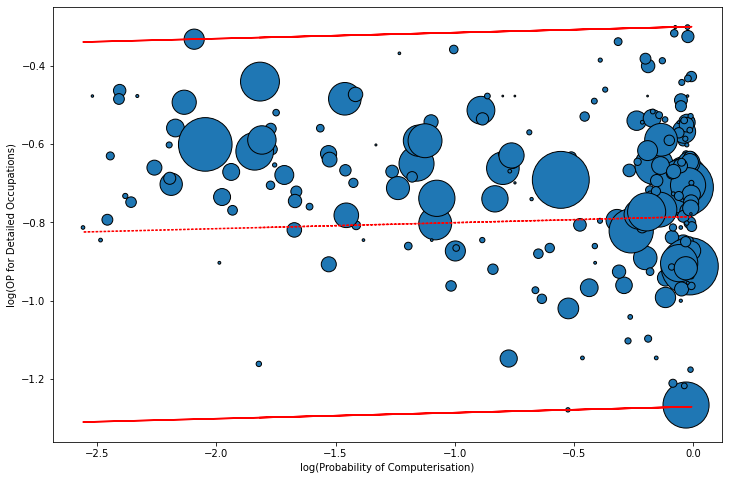
\includegraphics[width=15cm]{Figures/pac.png}
	\caption{Plot of $\log_{10}$(EP)/$\log_{10}$(OP) (for each Detailed Occupation) against $\log_{10}$(PCom) with PAC Learning applied ($x_{1}=0.485, x_{2}=0.0153, x_{3}=-0.785$). The red solid lines represents the boundaries of $H_{m}$ while the red dotted line is the median line. We can see that $H_{m}$ contains all of our datapoints while ensuring that the vertical width is minimised.}
	\label{fig:pac}
\end{figure}

Using Equation \ref{eq:4} and $\epsilon=0.01$, we calculate that $\mathbb{P}^{m} \{\delta_{1},...,\delta_{m}: \mathbb{P}(\delta \in \Delta: g(x^{*}_{m},\delta) > 0) \leq \epsilon \}$ is at least 0.407. This means that we are 40.7\% confident that there is at most a 1\% chance that a new sample falls outside of our hypothesis $H_{m}$ in Figure \ref{fig:pac}. The confidence lower bounds for other values of $\epsilon$ are shown in Table \ref{tab:confidence}. The confidence shoots up to almost 100\% with just an $\epsilon$ value of 0.05. This is not too surprising given that $H_{m}$ covers a relatively huge area.

\begin{table}[]
\centering
\begin{tabular}{l|l}
\textbf{$\epsilon$} & \textbf{$1-q(m,\epsilon)$} \\ \hline
0.01             & 0.4070228538 \\ \hline
0.05             & 0.9993799909 \\ \hline
0.10             & 0.9999999905
\end{tabular}
\caption{Confidence lower bound for corresponding $\epsilon$ values when using all samples.}
\label{tab:confidence}
\end{table}


While $H_{m}$ contains all of our datapoints while keeping $x_{1}$ minimised, it is not very useful since it ignores the underlying downward trend. In fact, $H_{m}$ would suggest a slight upward trend. This is because we have included the outlier datapoints (relative to the downward trend) in our set $S$. Hence, it would be useful to be able to apply PAC Learning to a dataset with discarded samples. Fortunately, \cite{kostas} details such an approach with a specific scenario discarding scheme.

Using scenario program \ref{eq:2} as reference, let us assume that $x^{*}_{m}$ exists and is unique, and that the scenario program is fully-supported. We then discard the support set for $x^{*}_{m}$. This will correspond to removing $n_{x}$ constraints since we assumed that the program is fully-supported. We are then left with a new scenario program with $m-n_{x}$ number of constraints. Assuming the optimiser for this new program exists and is unique, and that this new program is also fully-supported, we can repeat the discarding process to obtain a third scenario program with $m-2n_{x}$ constraints. We can repeat this $k$ number of times, removing $r=kn_{x}$ constraints in total and leaving us with a scenario program with $m-kn_{x}$ constraints. Hence, we get the following:

\begin{equation}
	\label{eq:6}
	q(m,\epsilon) = \sum_{i=0}^{r+n_{x}-1}{m \choose i}\epsilon^{i}(1-\epsilon)^{m-i}.
\end{equation}

Note that we assumed above that all $k$ new scenario programs obtained through this discarding scheme are fully-supported. Even if this assumption does not hold, we can introduce a lexicographic order as a way to select which constraints to discard, in which case we can still use the above result provided that all the $k$ new scenario programs as well as the original program are non-degenerate (recall that fully-supported implies non-degenerate, but not the other way around).

By assuming $x^{*}_{m-j}$ for our scenario program \ref{eq:5} is unique for $j=n_{x},2n_{x},...,kn_{x}$, and that the scenario program is at least non-degenerate, we can apply the above scenario discarding scheme as a way of excluding outlier datapoints. Figure \ref{fig:pac2} shows the plots for various values of $r$.



\begin{figure}[!htb]
	\centering
	\subfloat[$r=15 (x_{1}=0.386, x_{2}=-0.0292, x_{3}=-0.774)$]{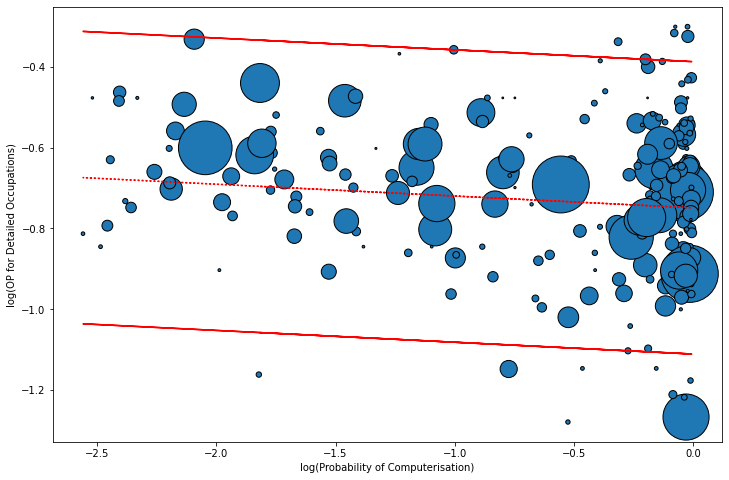
\includegraphics[width=15cm]{Figures/pac5.png}\label{fig:pac5}}
	\hfill
	\subfloat[$r=30$ $(x_{1}=0.274,x_{2}=0.0140,x_{3}=-0.716)$]{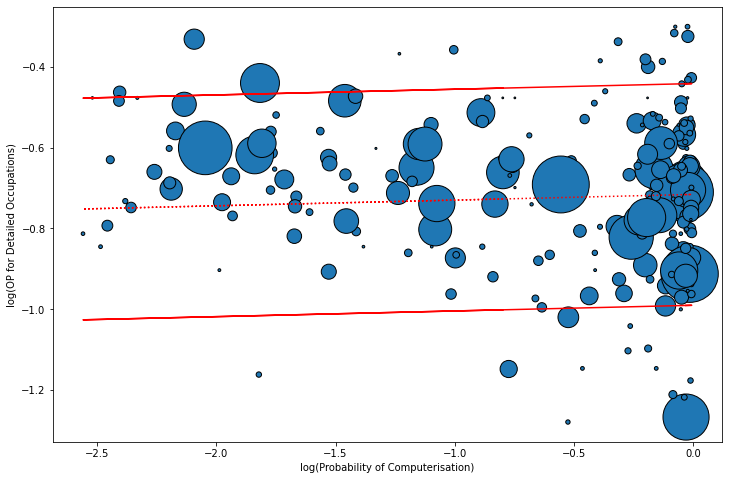
\includegraphics[width=15cm]{Figures/pac10}\label{fig:pac10}}
	\hfill
\end{figure}

\begin{figure}[!htb]
    \ContinuedFloat
 	\subfloat[$r=45$ $(x_{1}=0.242, x_{2}=-0.0142, x_{3}=-0.730)$]{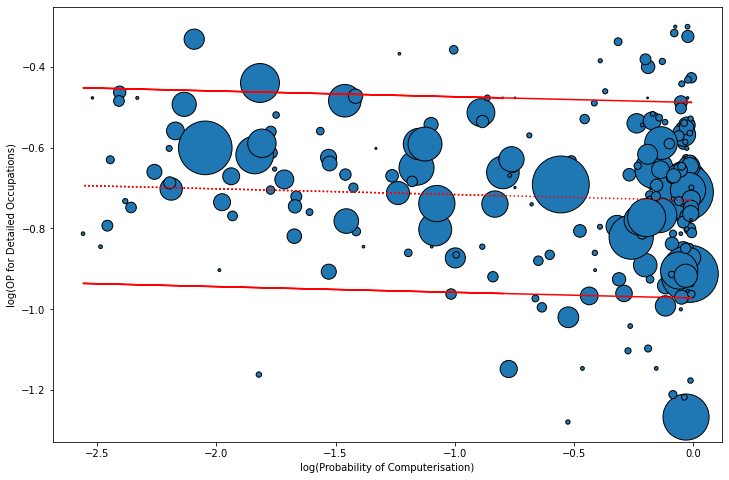
\includegraphics[width=15cm]{Figures/pac15}\label{fig:pac15}}
	\hfill	
    \subfloat[$r=60$ $(x_{1}=0.208, x_{2}=-0.0304, x_{3}=-0.737)$]{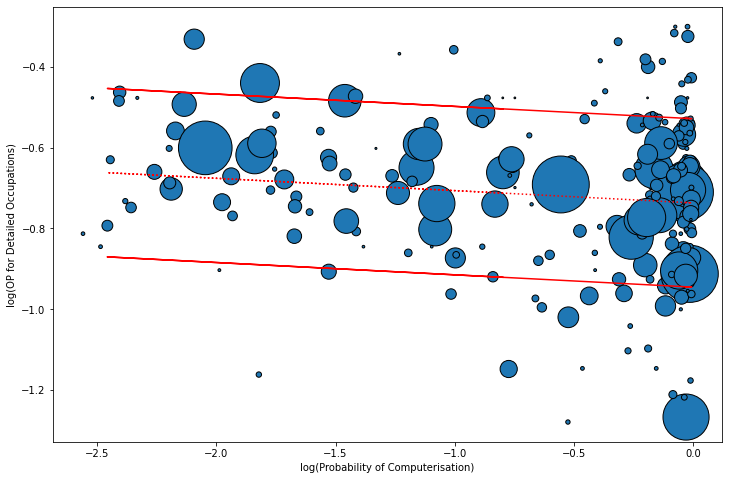
\includegraphics[width=15cm]{Figures/pac20}\label{fig:pac20}}
	\hfill
	\caption{Plot of $\log_{10}$(EP)/$\log_{10}$(OP) (for each Detailed Occupation) against $\log_{10}$(PCom) with PAC Learning and scenario discarding scheme applied. The red solid lines represents the boundaries of $H_{m}$ while the red dotted line is the median line. We can see $H_{m}$ starts to reflect the downward trend that we identified in the data. $x_{1}$ also gets smaller as $r$ increases, which corresponds to the decreasing vertical distance between the two red boundary lines.}
	\label{fig:pac2}
\end{figure}


For $r=60$, we can see that $H_{m-60}$ has been constrained to the collection of datapoints that we think are inliers. 60 discarded datapoints may seem like a lot, but those 60 occupations only represent $12.9\%$ of the total number of employed people present in \emph{joint\_auto} in 2012. This means that a large proportion of the employed people represented in our dataset are captured within $H_{m-60}$. Using Equation \ref{eq:6}, we can calculate the lower bounds for our confidence for various values of $\epsilon$ when $r=60$ (Table \ref{tab:confidence2}).

\begin{table}[]
\centering
\begin{tabular}{l|l}
\textbf{$\epsilon$} & \textbf{$1-q(m,\epsilon)$} \\ \hline
0.01             & $2.331468\times10^{-15}$ \\ \hline
0.05             & 0.001427 \\ \hline
0.10             & 0.540832 \\ \hline
0.15             & 0.990461 \\ \hline
0.20             & 0.999988
\end{tabular}
\caption{Confidence lower bound for corresponding $\epsilon$ values when $r=60$.}
\label{tab:confidence2}
\end{table}

While we can be almost 100\% certain that at least 99\% of new datapoints will lie outside $H_{m-60}$ (which is not great), we can be at least 50\% sure that at most 10\% of new datapoints will lie outside $H_{m-60}$ and pretty much 100\% confident that at most 15\% of new datapoint will lie outside $H_{m-60}$.

\subsubsection*{Conclusion}
In this section, we discussed the basic theory behind PAC Learning, and applied it on our dataset. We then noted that the presence of potential outliers were affecting the performance of our PAC Learning model and introduced the concept of a scenario discarding scheme that was devised for control problems. We then used this scheme as a way of excluding outliers from our model and showed that some of our confidence lower bounds were still decent. In doing so, we have demonstrated the viability of using these techniques to build a minimum region of confidence for any dataset (recall that nowhere have we made any assumptions about the underlying probability distribution).

\clearpage

\section{Conclusion}
In this report, we attempt to examine the relationship between automation and age distribution within occupations. To do so, we took age distribution data from the US Bureau of Labor Statistics and standardised all of it according to the 2018 Standard Occupational Classification system, and mapped it to the dataset containing Probability of Computerisation values from \cite{osborne2017future}. This gave us a joint standardised dataset covering the year 2011 to 2021, which may be useful to others doing related works. We also found that there was a general trend of ageing across most occupations. We then explored trends within this joint dataset but found no significant trends for the most part. Based on this, we conclude that governments cannot expect that the loss of jobs from automation will cancel out the lack of workers in the labour force due to an ageing population, and we recommend that they take more active steps towards addressing these issues.

That being said, we did discover a possible trend: an inverse relationship between the proportion of 55 and older workers within an occupation and the Probability of Computerisation of that occupation. We applied weighted least squares, Bayesian ridge, and Random Sample Consensus regression to this set of variables. Given the high variance around the regression lines, we wondered if we could instead construct a region that we have high confidence would contain a high percentage of new datapoints. To do so, we turned to Probably Approximately Correct learning, and used it in conjunction with a scenario discarding scheme originally devised for optimisation programs within control problems. This allowed us to construct the region while excluding some outliers. We concluded that it was possible to construct a region for which we are almost 100\% confident would contain at least 85\% of new datapoints. This also acts as a proof of concept of using such a technique on datasets with high variance.


\subsection*{Future extensions}

\clearpage

\printbibliography[heading=bibintoc]


\end{document}